\documentclass[12pt,a4paper]{report}

%%------------------------------- preamble ------------------------------------

%% comment next for EN
\usepackage[english]{babel}      % language PT 
\usepackage[utf8]{inputenc}       % accents
\usepackage[T1]{fontenc}          % PS fonts
% \usepackage{newtxtext,newtxmath}  % do not use CM fonts
% \usepackage{mathpazo}
\usepackage{XCharter}
\usepackage[xcharter]{newtxmath}
\usepackage{amsmath}              % multi-line and other mathematical statements
\usepackage{setspace}             % setting the spacing between lines
\usepackage{graphicx}             % go far beyond what the graphics package
\usepackage[normalem]{ulem}       % various types of underlining
\usepackage{caption}              % rotating captions, sideways captions, etc.
\usepackage{float}                % tables and figures in the multi-column environment 
\usepackage{subcaption}           % for subfigures and the like
\usepackage{longtable}            % tables that continue to the next page
\usepackage{multirow}             % tabular cells spanning multiple rows
\usepackage[table]{xcolor}        % driver-independent color extensions
\usepackage{lipsum}               % loren dummy text
\setlength{\marginparwidth}{2cm}  % todonotes' requirements
\usepackage{todonotes}            % todo's
\usepackage{csquotes}             % context sensitive quotation facilities
\usepackage[backend=biber,authordate]{biblatex-chicago}  % Chicago Manual of Style
\usepackage{pgfgantt}             % Gantt charts
\usepackage[breakable, listings, skins]{tcolorbox}
\usepackage{eurosym}
\usepackage{booktabs}

%% document dimensions
\usepackage[a4paper,left=25mm,right=25mm,top=25mm,bottom=25mm,headheight=6mm,footskip=12mm]{geometry}
\setlength{\parindent}{0em}
\setlength{\parskip}{1ex}

%% headers & footers
\usepackage{lastpage}
\usepackage{fancyhdr}
\fancyhf{}                            % clear off all default fancyhdr headers and footers
\rhead{\small{\emph{\projtitle, \projauthor}}}
\rfoot{\small{\thepage\ / \pageref{LastPage}}}
\pagestyle{fancy}                     % apply the fancy header style
\renewcommand{\headrulewidth}{0.4pt}
\renewcommand{\footrulewidth}{0.4pt}

%% colors
\usepackage{color}
\definecolor{engineering}{rgb}{0.549,0.176,0.098}
\definecolor{cloudwhite}{cmyk}{0,0,0,0.025}

%% source-code listings
\usepackage{listings}
\lstset{ %
 language=C,                        % choose the language of the code
 basicstyle=\footnotesize\ttfamily,
 keywordstyle=\bfseries,
 numbers=left,                      % where to put the line-numbers
 numberstyle=\scriptsize\texttt,    % the size of the fonts that are used for the line-numbers
 stepnumber=1,                      % the step between two line-numbers. If it's 1 each line will be numbered
 numbersep=8pt,                     % how far the line-numbers are from the code
 frame=tb,
 float=htb,
 aboveskip=8mm,
 belowskip=4mm,
 backgroundcolor=\color{cloudwhite},
 showspaces=false,                  % show spaces adding particular underscores
 showstringspaces=false,            % underline spaces within strings
 showtabs=false,                    % show tabs within strings adding particular underscores
 tabsize=2,                         % sets default tabsize to 2 spaces
 captionpos=t,                      % sets the caption-position to top
 belowcaptionskip=12pt,             % space between caption and listing
 breaklines=true,                   % sets automatic line breaking
 breakatwhitespace=false,           % sets if automatic breaks should only happen at whitespace
 escapeinside={\%*}{*)},            % if you want to add a comment within your code
 morekeywords={*,var,template,new}  % if you want to add more keywords to the set
}

%% hyperreferences (HREF, URL)
\usepackage{hyperref}
\hypersetup{
    plainpages=false, 
    pdfpagelayout=SinglePage,
    bookmarksopen=false,
    bookmarksnumbered=true,
    breaklinks=true,
    linktocpage,
    colorlinks=true,
    linkcolor=engineering,
    urlcolor=engineering,
    filecolor=engineering,
    citecolor=engineering,
    allcolors=engineering
}

\newtcblisting{htmlcode}{
    arc=2pt, outer arc=2pt, boxrule=0.5pt, breakable,
    colback=gray!5, colframe=gray!60!black,
    listing only, top=0pt, bottom=0pt, middle=1pt, boxsep=3pt,
    listing options={
        basicstyle=\footnotesize\ttfamily, numbers=none, breaklines=true,
        language=HTML, tabsize=2, extendedchars=true,
        literate={€}{{\euro}}1 {é}{{\'e}}1 {â}{{\^a}}1 {à}{{\`a}}1 {ô}{{\^o}}1 {ê}{{\^e}}1,
    },
    title=\textbf{Parsed HTML Output}, fonttitle=\small\sffamily,
    colbacktitle=gray!20!white, coltitle=black, enhanced, width=\textwidth, right=5mm,
}

%% path to the figures directory
\graphicspath{{figures/}}

%% bibliography file, must be in preamble
\addbibresource{bibliography.bib}
\defbibheading{webography}{\section*{Webography}}
\DeclareSourcemap{
  \maps[datatype=bibtex]{
    \map{
      \step[typesource=online, typetarget=online, final]
      \step[fieldset=keywords, fieldvalue=webography]
    }
  }
}

%% macros, to be updated as needed
\newcommand{\school}{Institut National des Sciences Appliquées de Toulouse }
\newcommand{\degree}{Bachelor's Degree in Computer Science and Engineering}
\newcommand{\projtitle}{Optimizing and Adapting Language Models for Domain-Specific Task}
\newcommand{\subtitle}{End-of-studies Apprenticeship Report}
\newcommand{\projauthor}{Minh Duy Nguyen}
\newcommand{\supervisor}{Milad Mozafari (Torus AI), David Bertoin (INSA Toulouse)}
\newcommand{\tutor}{David Bertoin}

%% my other macros, if needed
\newcommand{\windspt}{\textsf{WindsPT\/}}
\newcommand{\windscannerpt}{\emph{Windscanner.PT\/}}
\newcommand{\class}[1]{{\normalfont\sffamily #1\/}}
\newcommand{\svg}{\class{SVG}}

%% my environments for infos
\newenvironment{info}[1]{\vspace*{6mm}\color{blue}[ \textbf{INFO:} \begin{em} #1}
                        {\vspace*{3mm}\end{em} ]}
\newenvironment{infoopt}[1]{\vspace*{6mm}\color{blue}[ \textbf{INFO (optional element):} \begin{em} #1}
                        {\vspace*{3mm}\end{em} ]}

%%------------------------------- document-------------------------------------

\begin{document}

%% preamble page numbers with roman numerals
\pagenumbering{roman}\setcounter{page}{1}
\pagestyle{plain}

%%------------------------------- cover page ----------------------------------

\begin{titlepage}
\center

%% --- Phần Header chia 2 cột ---
\begin{minipage}[t]{0.32\textwidth}
    \begin{flushleft} 
        \centering
        \textbf{\large INSA Toulouse}\\
        \small \textit{Department of Mathematics and Modelling}
    \end{flushleft}
\end{minipage}
\hfill
\begin{minipage}[t]{0.32\textwidth}
    \begin{flushright} 
        \centering
        \textbf{\large Torus AI}\\
        \small \textit{TorusLab -- Research \& Development Division} % Bạn có thể sửa thông tin này
    \end{flushright}
\end{minipage}
\hfill
\begin{minipage}[t]{0.32\textwidth}
    \begin{flushright} 
        \centering
        \textbf{\large ENSEEIHT}\\
        \small \textit{Department of Computer Science and Digital Technology} % Bạn có thể sửa thông tin này
    \end{flushright}
\end{minipage}

%% --- Phần Logo (Dàn hàng ngang 3 logo) ---
%% Lưu ý: Bạn cần đảm bảo có file logo của Torus AI trong thư mục figures
\begin{figure}[H]
    \centering
    \begin{minipage}{0.3\textwidth}
        \centering
        \includegraphics[width=\textwidth]{figures/logo-INSA.png}
    \end{minipage}
    \hfill
    \begin{minipage}{0.3\textwidth}
        \centering
        % Thay 'logo-torus' bằng tên file logo công ty bạn
        \includegraphics[width=0.8\textwidth]{figures/logo-torus.png} 
    \end{minipage}
    \hfill
    \begin{minipage}{0.3\textwidth}
        \centering
        \includegraphics[width=\textwidth]{figures/logo-N7.png}
    \end{minipage}
\end{figure}

\vfill

{\large \textbf{\subtitle}}\\
\vfill 
\rule{\linewidth}{1pt} \\[0.5cm]
{\Huge \textbf{\projtitle}}\\
\rule{\linewidth}{1pt} \\[0.5cm]

% {\Large \textbf{\projauthor}}

%% --- Khoảng cách sau phần tiêu đề ---
\vspace{2cm}

%% --- Cột Author và Supervised by ---
\begin{minipage}[t]{0.45\textwidth}
    \begin{flushleft}
      \centering 
        \textit{Author:}\\
        \textbf{\projauthor}
    \end{flushleft}
\end{minipage}
\hfill
\begin{minipage}[t]{0.48\textwidth}
    \begin{flushleft}
      \centering
        \textit{Supervised by:}\\
        Milad Mozafari (Torus AI)\\
        David Bertoin (INSA Toulouse)
    \end{flushleft}
\end{minipage}

\vspace{2cm}

%% --- Phần Hội đồng Jury ---
\begin{center}
    \textit{Defended on February 5, 2026, in front of the jury composed of :} \\[0.4cm]
    \begin{tabular}{lll}
        Mr. David Bertoin    & INSA Toulouse & -- Reporter \\
        Mr. Charles Dossal &  INSA Toulouse & -- Examiner \\
        Mr. Olivier Roustant   & INSA Toulouse & -- Examiner \\
    \end{tabular}
\end{center}

\vfill

%% --- Năm học ---
\begin{center}
    Academic year: 2025-2026
\end{center}

%% --- Dòng chữ Confidential (Đỏ) ---
\begin{flushright}
    \begin{tcolorbox}[
        enhanced,                   % Kích hoạt các tính năng nâng cao
        colframe=red,       % Màu khung là màu đỏ nâu 'engineering' bạn đã tạo
        colback=white,              % Màu nền bên trong hộp là trắng
        coltext=red,        % Màu chữ cũng là đỏ nâu
        boxrule=2pt,                % Độ dày của đường viền khung
        arc=0mm, outer arc=0mm,     % Đặt góc bo tròn bằng 0 để tạo góc vuông
        fontupper=\Large\bfseries,  % Cỡ chữ to (\Large) và đậm (\bfseries)
        halign=center,              % Căn giữa chữ trong khung
        width=6.5cm,                % Chiều rộng của khung
        boxsep=4pt                  % Khoảng cách từ chữ đến viền khung
    ]
        CONFIDENTIAL
    \end{tcolorbox}
\end{flushright}

\end{titlepage}

%%------------------------------- Abstract ------------------------------------

\chapter*{Abstract}
Large Language Models (LLMs) have demonstrated remarkable capabilities in natural language understanding and generation. However, deploying these models in enterprise environments faces two fundamental challenges: the \textit{Knowledge Gap}, arising from static training data and hallucination risks, and the \textit{Behavior Gap}, stemming from difficulties in precisely controlling model behavior for specialized tasks.

This report presents two complementary approaches developed during an apprenticeship at Torus AI to address these challenges. First, we propose an Advanced Multimodal RAG (Retrieval-Augmented Generation) pipeline for complex document understanding in financial and healthcare domains. Through systematic improvements including structure-preserving parsing, semantic enrichment via multimodal summarization, and multi-layer retrieval combining hybrid search with cross-encoder reranking, we achieved a 32.8\% improvement in answer precision over baseline methods.

Second, we investigate Parameter-Efficient Fine-Tuning (PEFT) techniques to adapt Small Language Models (SLMs) for persona-based conversational tasks. Using behavioral knowledge distillation from GPT-4o and Qwen-Plus, we fine-tuned Qwen2.5-1.5B-Instruct with and without LoRA to create a Tarot Reader chatbot. Evaluation results demonstrate that the fine-tuned 1.5B model achieved behavioral consistency surpassing GPT-4 with prompt engineering (71\% vs 25\% win rate in human evaluation), while reducing operational costs by 80--90\% and achieving sub-100ms latency suitable for real-time deployment.

These findings contribute practical frameworks for deploying domain-specific AI applications under enterprise constraints, demonstrating that both knowledge accuracy and behavioral consistency can be achieved through targeted optimization rather than model scaling.

\vspace{1cm}
\textbf{Keywords:} Large Language Models, Retrieval-Augmented Generation, Parameter-Efficient Fine-Tuning, LoRA, Knowledge Distillation, Multimodal Document Understanding, Small Language Models, Behavioral Adaptation, Enterprise AI Deployment


%\vspace{\fill}
%{\Large \textbf{Palavras-chave}:} palavra1, palavra2, palavra3, palavra4
%\vspace*{24mm}

%%------------------------------- Acknowledgments -----------------------------

\chapter*{Acknowledgement}

- Milad, Thao, Erfan, Khoi, Davis, Zung
- TorusLab, Torus AI, 
- 

%%------------------------------- table of contents ---------------------------

%% redefine tableofcontents text, ONLY for PT
\renewcommand{\contentsname}{Table of contents}

\tableofcontents


%%------------------------------- Glossary ------------------------------------

% \chapter*{Figures and tables}
% \addcontentsline{toc}{chapter}{List of Figures and Tables}

%% ==================== LIST OF FIGURES ====================
% \section*{List of Figures}
% \addcontentsline{toc}{section}{List of Figures}

\listoffigures

%% ==================== LIST OF TABLES ====================
% \section*{List of Tables}
% \addcontentsline{toc}{section}{List of Tables}

\listoftables

\newpage
%%------------------------------- chapter ------------------------------------

\chapter{Introduction}

%% display headers & footers
\pagestyle{fancy}
%% main page numbers with arabic numerals
\pagenumbering{arabic}\setcounter{page}{1}

\section{General Context}

\subsection{Evolution of Large Language Model}

Over the past decade, the fields of Artificial Intelligence (AI) and Natural Language Processing (NLP) have witnessed groundbreaking advances, particularly since the emergence of the Transformer architecture \parencite{vaswani2017attention}. Large Language Models (LLMs) such as GPT-4 \parencite{achiam2023gpt}, Claude \parencite{anthropic2024claude}, Gemini \parencite{comanici2025gemini}, and open-source models like Llama 3 \parencite{grattafiori2024llama} and Qwen 2 \parencite{team2024qwen2} have demonstrated superior capabilities in understanding context, generating text, and performing logical inference across a variety of tasks.

\subsection{The Research-Industrial Application Gap}

Transferring language models from the research environment to practical industrial applications faces significant challenges. Indeed, according to an MIT survey, up to 95\% of AI generation/LLM projects in enterprises do not generate significant profit and loss (P\&L) impact---reflecting that the majority of businesses struggle to move LLMs from pilot to production deployment \parencite{tomshardware2024mit}. Additionally, other surveys show that approximately 72\% of businesses encounter at least one barrier to adopting GenAI (including operating costs, governance, and model accuracy), and over 50\% consider accuracy a major barrier to LLM deployment \parencite{writer2024survey}.

Although Foundation Models possess a vast amount of general knowledge, they often encounter two serious limitations when solving domain-specific tasks:


\subsubsection{Knowledge Gap}

In critical fields such as healthcare, finance, and insurance, information is often contained in complex documents (financial reports, medical technical catalogs) and changes constantly. LLMs face three main problems:

\begin{itemize}
\item Static Knowledge: Model knowledge is limited by the training time (knowledge cutoff), making it impossible to update new information without retraining. 
\item  Private Data Inaccessibility: The model cannot access confidential organizational documents such as contracts, internal procedures, or patient records.
\item Hallucination: LLMs tend to confidently generate false information \parencite{ji2023hallucination, huang2023hallucination_survey} which is unacceptable in medical or financial decisions where near-absolute accuracy is required.
\end{itemize}

\subsubsection{Efficiency \& Behavior Gap}

For tasks that require strict adherence to a predefined behavioral scenario, a specific linguistic style (e.g., psychological counselor or analyst), or deployment under constrained hardware environments, extremely large language models with hundreds of billions of parameters are often neither cost-effective nor latency-efficient. As shown by the compute-optimal scaling analysis of \textcite{hoffmann2022chinchilla}, increasing model size without proportionally increasing training data leads to inefficient use of compute, resulting in substantially higher training and inference costs. Furthermore, the scaling laws identified by \textcite{kaplan2020scaling} demonstrate that model performance improves as a power-law function of compute, implying that compute—and consequently deployment cost and latency—grows rapidly with model size, limiting the practicality of massive models for many real-world enterprise settings.

\subsection{Research motivation}

Based on the above reality, this report focuses on researching and implementing advanced techniques to \textbf{optimize and adapt Language Models for specific data domains}, with two main approaches:

\begin{itemize}
  \item Retrieval-Augmented Generation (RAG): Integrating external knowledge bases to address the Knowledge Gap.
  \item Parameter-Efficient Fine-Tuning (PEFT): Adapting model behavior to address the Behavior Gap.
\end{itemize}


\section{Internship Environment}

This master's report was completed at \textbf{Torus AI}, a technology company with the mission \textit{Intelligence for Life}, specializing in providing advanced AI solutions to improve quality of life and business efficiency.

I worked in the Research and Development Team (R\&D Team - Torus Lab) as a Machine Learning Engineer Alternant. At Torus AI, the R\&D department acts as a bridge between the latest academic research (State-of-the-Art) and commercial products. The team's main task is to continuously explore emerging Generative AI technologies, assess their feasibility, and build functional prototypes (PoCs) to verify their effectiveness before integration into the main product system.

The R\&D work environment demands flexible thinking: not just using existing APIs, but delving into customizing architecture, optimizing data processing pipelines, and quantitatively evaluating technical solutions.

My role in the R\&D department includes:

\begin{itemize}
  \item Researching emerging Generative AI technologies
  \item Evaluating feasibility and building functional prototypes (PoCs)
  \item Integrating solutions into product systems
\end{itemize}

Resources provided:

\begin{itemize}
  \item GPU infrastructure: NVIDIA RTX 3090 (24GB)
  \item Real-world enterprise data: Medical documents (CCAM), insurance financial reports
  \item API access: OpenAI GPT-4, Google Gemini, Qwen API
\end{itemize}

\section{Problem Statement}

During our work in the R\&D department, we identified two core problems that needed to be addressed when applying GenAI in practice, corresponding to two main technical approaches:

\subsubsection{Problem 1: Integration of External Knowledge from Complex Unstructured Data}

Partner businesses (such as insurance companies, healthcare facilities) possess large amounts of data in the form of PDF documents containing text, tables, and images. Traditional RAG methods based on plain text (text-only) fail to understand the semantics of complex tables or visual information \parencite{gao2023rag_survey, li2024multimodal_rag}.
The question is: How to build a Multimodal RAG pipeline capable of accurately parsing, indexing, and retrievaling information from these mixed documents to support decision-making (e.g., medical refund code lookup, financial data analysis)?

\subsubsection{Problem 2: Behavioral Adaptation and Resource Optimization for Small Models (Behavioral Adaptation \& Efficiency)}

For applications requiring high interactivity, counseling, or entertainment (such as psychological counseling chatbots or Tarot Readers), the requirement is not only for information accuracy but also for consistency in tone and style and rule-based reasoning. Using large models (like GPT-4) via APIs is both costly to operate and difficult to fully control behavior.

Recent research has shown that small language models can achieve competitive performance through efficient fine-tuning techniques like LoRA \parencite{hu2022lora} and QLoRA \parencite{dettmers2024qlora}, combined with synthetic data generation approaches \parencite{taori2023alpaca, wang2023selfinstruct}.

The question is: Is it possible to fine-tune small language models (such as Qwen, Llama < 7B parameters) using parameter optimization techniques (PEFT/LoRA) and quantization so that they achieve inference capabilities and writing styles comparable to large models, but can be run locally at low cost?

\section{Objectives and expected results}

This report aims to achieve the following objectives:

\begin{enumerate}
  \item Design and implement an Advanced Multimodal RAG pipeline capable of accurately extracting and retrieving information from complex documents containing text, tables, and images in the medical and financial domains.

  \item Develop a methodology for fine-tuning Small Language Models (< 2B parameters) using PEFT/LoRA techniques to achieve domain-specific behavior adaptation while enabling cost-effective local deployment.

  \item Establish \textbf{systematic evaluation frameworks} for both RAG retrieval quality using RAGAS metrics \parencite{es2024ragas} and fine-tuned model performance using LLM-as-a-Judge approaches \parencite{zheng2023llmjudge}, enabling reproducible benchmarking.

\end{enumerate}


\section{Report structure}
	
In addition to this introduction, this report is organized into four main chapters and appendices. Chapter 2 provides the theoretical background, introducing the foundational concepts of Retrieval-Augmented Generation (RAG) and Parameter-Efficient Fine-Tuning (PEFT), followed by an overview of Knowledge Distillation and Synthetic Data Generation techniques. Chapter 3 addresses the Knowledge Gap by presenting an Advanced Multimodal RAG pipeline for processing complex medical and financial documents. Chapter 4 tackles the Behavior Gap through LoRA fine-tuning of small Qwen models for persona-based tasks. Chapter 5 concludes the report by summarizing contributions and proposing future research directions. The Appendices provide supplementary materials including prompt templates and training configurations.

%%------------------------------- CHAPTER 2: THEORETICAL BACKGROUND ------------------------------------

\chapter{Theoretical Background}

As introduced in Chapter 1, deploying Large Language Models (LLMs) in enterprise environments faces two fundamental challenges: the \textit{Knowledge Gap} stemming from static training data and hallucination risks, and the \textit{Behavior Gap} arising from the difficulty in precisely controlling model behavior for specialized tasks. This chapter establishes the theoretical foundations for two complementary approaches to address these challenges: Retrieval-Augmented Generation (RAG) for knowledge integration, and Parameter-Efficient Fine-Tuning (PEFT) for behavioral adaptation. Additionally, we discuss Knowledge Distillation and Synthetic Data Generation---techniques that enable the transfer of capabilities from large models to smaller, more deployable ones.

\section{Retrieval-Augmented Generation (RAG)}

\subsection{Motivation and Core Concept}

Despite their impressive capabilities, LLMs suffer from inherent limitations that restrict their applicability in knowledge-intensive domains \autocite{lewis2020retrieval}. These limitations include: (1) \textit{knowledge cutoff}---the model cannot access information beyond its training date; (2) \textit{hallucination}---the tendency to generate plausible but factually incorrect content \autocite{ji2023survey}; and (3) \textit{lack of attribution}---inability to cite sources for generated claims.

Retrieval-Augmented Generation addresses these issues by augmenting the LLM's input with relevant documents retrieved from an external knowledge base. Instead of relying solely on parametric knowledge (stored in model weights), RAG combines it with non-parametric knowledge (retrieved documents), enabling the model to ground its responses in verifiable sources \autocite{lewis2020retrieval}.

The fundamental insight behind RAG is that while LLMs excel at language understanding and generation, they need not memorize all factual knowledge in their parameters. By decoupling knowledge storage (in a retrievable database) from language capabilities (in the model), RAG achieves both factual accuracy and generative fluency.

\subsection{Basic RAG Pipeline Architecture}

A standard RAG pipeline consists of two main phases: an offline \textbf{Indexing Phase} and an online \textbf{Query Phase} \autocite{gao2024retrievalaugmented}. Figure \ref{fig:basic_rag_pipeline} illustrates the a RAG architecture.

\begin{figure}[H]
    \centering
    \includegraphics[width=0.85\textwidth]{figures/basic_rag_pipeline.png}
    \caption{Basic RAG Pipeline Architecture showing Indexing Phase (offline) and Query Phase (online)}
    \label{fig:basic_rag_pipeline}
\end{figure}

\subsubsection{Indexing Phase}

The indexing phase prepares the knowledge base for efficient retrieval:

\begin{enumerate}
    \item \textbf{Document Loading}: Raw documents (PDFs, web pages, databases) are ingested into the system.
    
    \item \textbf{Chunking}: Documents are split into smaller segments called \textit{chunks}. The chunk size represents a trade-off: smaller chunks enable more precise retrieval but may lose context, while larger chunks preserve context but reduce retrieval granularity. Common strategies include fixed-size chunking (e.g., 512 tokens with overlap) and semantic chunking based on document structure \autocite{liu2024lost}.
    
    \item \textbf{Embedding}: Each chunk is transformed into a dense vector representation using an embedding model. These vectors capture semantic meaning, allowing similar concepts to have proximate representations in vector space. Popular models include OpenAI's text-embedding-ada-002, Sentence-BERT \autocite{reimers2019sentence}, and multilingual variants like E5 \autocite{wang2024multilingual}.
    
    \item \textbf{Indexing}: Embeddings are stored in a vector database (e.g., ChromaDB, Pinecone, Qdrant) optimized for similarity search using algorithms like HNSW (Hierarchical Navigable Small World) or IVF (Inverted File Index) \autocite{malkov2020efficient}.
\end{enumerate}

\subsubsection{Query Phase}

When a user submits a query, the system executes the following steps:

\begin{enumerate}
    \item \textbf{Query Embedding}: The user query is embedded using the same model used during indexing, ensuring comparable vector representations.
    
    \item \textbf{Retrieval}: The system performs similarity search (typically using cosine similarity or dot product) to find the $k$ most relevant chunks. This is often called Dense Retrieval or Vector Search.
    
    \item \textbf{Augmentation}: Retrieved chunks are concatenated with the original query to form an augmented prompt. A typical template might be:
    
    \begin{quote}
    \texttt{Context: [retrieved chunks]\\
    Question: [user query]\\
    Answer the question based on the context above.}
    \end{quote}
    
    \item \textbf{Generation}: The augmented prompt is passed to the LLM, which generates a response grounded in the retrieved context.
\end{enumerate}

While conceptually elegant, basic RAG faces several challenges in practice such as \textbf{Loss of Document Structure}, \textbf{Chunking Artifacts}, \textbf{Retrieval Errors}, and the \textbf{Lost in the Middle} phenomenon \autocite{liu2024lost}. These limitations motivate advanced RAG techniques discussed in Chapter \ref{chapter:multimodal_rag}, including multimodal parsing, hybrid search, and reranking.

\section{Parameter-Efficient Fine-Tuning (PEFT)}

\subsection{The Fine-Tuning Paradigm}

While RAG addresses the Knowledge Gap by augmenting LLMs with external information, the \textit{Behavior Gap}---the difficulty in making models consistently adhere to specific communication styles, workflows, or personas---requires a different approach. Fine-tuning adapts pre-trained models to downstream tasks by continuing training on task-specific data, enabling the model to internalize desired behaviors into its parameters.

Traditional full fine-tuning updates all model parameters, which for modern LLMs with billions of parameters presents significant challenges:

\begin{itemize}
    \item \textbf{Computational Cost}: Training all parameters requires substantial GPU memory and compute time. For a 7B parameter model in FP16, storing model weights, gradients, and optimizer states requires approximately 112GB of memory.
    \item \textbf{Storage Overhead}: Each fine-tuned variant requires storing a complete copy of all model weights, making multi-task or multi-tenant deployments impractical.
    \item \textbf{Catastrophic Forgetting}: Aggressive fine-tuning can degrade the model's general capabilities acquired during pre-training.
\end{itemize}

Parameter-Efficient Fine-Tuning (PEFT) methods address these challenges by training only a small subset of parameters while keeping the majority of the pre-trained model frozen. This approach dramatically reduces memory requirements, enables efficient multi-task adaptation through swappable modules, and often provides implicit regularization against overfitting.

\subsection{Low-Rank Adaptation (LoRA)}

Among PEFT methods, Low-Rank Adaptation (LoRA) \parencite{hu2021lora} has emerged as the dominant technique due to its simplicity, effectiveness, and inference efficiency. LoRA's key insight is that the weight updates during fine-tuning exhibit low intrinsic dimensionality---meaning they can be effectively approximated by low-rank matrices.

\subsubsection{Mathematical Formulation}

For a pre-trained weight matrix $\mathbf{W}_0 \in \mathbb{R}^{d \times k}$, LoRA represents the weight update as a low-rank decomposition:
\[
\mathbf{W} = \mathbf{W}_0 + \Delta\mathbf{W} = \mathbf{W}_0 + \mathbf{B}\mathbf{A}
\]
where $\mathbf{B} \in \mathbb{R}^{d \times r}$ and $\mathbf{A} \in \mathbb{R}^{r \times k}$, with rank $r \ll \min(d, k)$.

\begin{figure}[H]
    \centering
    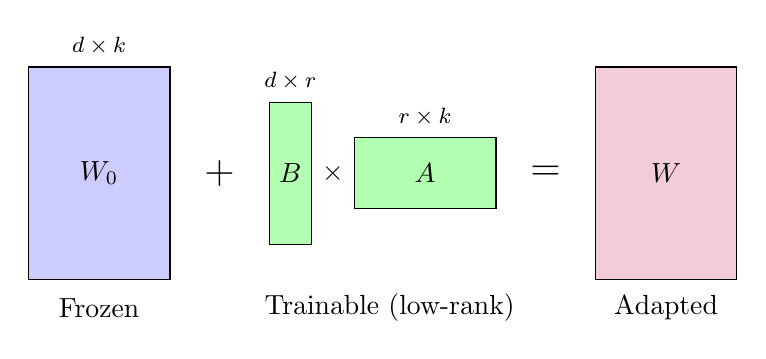
\begin{tikzpicture}[scale=0.9]
        % Original weight matrix
        \draw[fill=blue!20] (0,0) rectangle (2,3);
        \node at (1, 1.5) {$W_0$};
        \node at (1, -0.4) {Frozen};
        
        % Plus sign
        \node at (2.7, 1.5) {\Large $+$};
        
        % LoRA matrices
        \draw[fill=green!30] (3.4, 0.5) rectangle (4.0, 2.5);
        \node at (3.7, 1.5) {$B$};
        
        \node at (4.3, 1.5) {$\times$};
        
        \draw[fill=green!30] (4.6, 1.0) rectangle (6.6, 2.0);
        \node at (5.6, 1.5) {$A$};
        
        \node at (5.1, -0.4) {Trainable (low-rank)};
        
        % Equals sign
        \node at (7.3, 1.5) {\Large $=$};
        
        % Result
        \draw[fill=purple!20] (8,0) rectangle (10,3);
        \node at (9, 1.5) {$W$};
        \node at (9, -0.4) {Adapted};
        
        % Dimensions
        \node[font=\footnotesize] at (1, 3.3) {$d \times k$};
        \node[font=\footnotesize] at (3.7, 2.8) {$d \times r$};
        \node[font=\footnotesize] at (5.6, 2.3) {$r \times k$};
        
    \end{tikzpicture}
    \caption{LoRA: Low-Rank Adaptation. The original weight $W_0$ is frozen, while only the low-rank matrices $A$ and $B$ are trained.}
    \label{fig:lora_diagram}
\end{figure}

During training, $\mathbf{W}_0$ remains frozen while only $\mathbf{A}$ and $\mathbf{B}$ are updated. The forward pass becomes:
\[
\mathbf{h} = \mathbf{W}_0 \mathbf{x} + \frac{\alpha}{r} \mathbf{B}\mathbf{A}\mathbf{x}
\]
where $\alpha$ is a scaling hyperparameter that controls the magnitude of the adaptation.

\subsubsection{Parameter Efficiency Analysis}

The efficiency gains from LoRA are substantial. Consider applying LoRA to a weight matrix of dimensions $d \times k$:
\begin{itemize}
    \item Full fine-tuning: $d \times k$ trainable parameters
    \item LoRA with rank $r$: $r \times (d + k)$ trainable parameters
\end{itemize}

For a typical attention projection with $d = k = 4096$ and $r = 16$:
\begin{itemize}
    \item Full: $4096 \times 4096 = 16,777,216$ parameters
    \item LoRA: $16 \times (4096 + 4096) = 131,072$ parameters (0.78\% of full)
\end{itemize}

\subsubsection{Target Module Selection}

LoRA can be applied to any linear layer, but research and practice have identified attention projection matrices ($\mathbf{W}_Q$, $\mathbf{W}_K$, $\mathbf{W}_V$, $\mathbf{W}_O$) as particularly effective targets. Recent work has also demonstrated benefits from including feed-forward network (FFN) layers, especially for behavioral adaptation tasks where the model must learn new ``processing patterns'' rather than just new ``attention patterns.''

\subsubsection{Inference Efficiency}

A unique advantage of LoRA is that the adapted weights can be merged with the original weights after training:
\[
\mathbf{W}_{\text{merged}} = \mathbf{W}_0 + \mathbf{B}\mathbf{A}
\]
This merged model has identical architecture and inference cost to the original, with no additional latency overhead. Alternatively, keeping adapters separate enables efficient switching between different task-specific adaptations by swapping only the small LoRA matrices.

\subsection{Other PEFT Methods}

While LoRA dominates current practice, other PEFT approaches offer alternative trade-offs:

\textbf{Prefix Tuning} \parencite{li2021prefix}: Prepends trainable continuous vectors (``soft prompts'') to the input at each transformer layer. These prefixes learn to condition the frozen model's behavior without modifying its weights.

\textbf{Adapters} \parencite{houlsby2019adapter}: Insert small trainable bottleneck modules between transformer layers. Unlike LoRA, adapters add parameters to the forward pass, incurring slight inference overhead.

\textbf{QLoRA} \parencite{dettmers2023qlora}: Combines LoRA with 4-bit quantization, enabling fine-tuning of very large models on consumer hardware by dramatically reducing memory requirements.

Chapter \ref{chap:finetuning_slm_tarot} applies LoRA fine-tuning to adapt small language models for a specialized conversational task, demonstrating that behavioral consistency can be effectively learned with minimal parameter updates.


\section{Knowledge Distillation}

\subsection{Concept and Motivation}

Knowledge Distillation (KD) is a model compression technique that transfers knowledge from a large ``teacher'' model to a smaller ``student'' model \autocite{hinton2015distilling}. The motivation is that large models, while powerful, are often impractical for deployment due to latency, memory, and cost constraints. Distillation enables the student to achieve performance approaching the teacher while being significantly more efficient.

The key insight of \textcite{hinton2015distilling} is that the teacher's soft probability distribution contains richer information than hard labels. For example, when classifying an image of a dog, the teacher might output $P(\text{dog})=0.7, P(\text{wolf})=0.2, P(\text{cat})=0.1$. These ``dark knowledge'' probabilities reveal that the image has wolf-like features---information lost in the hard label ``dog''.

\subsection{Distillation Objective}

The student is trained to minimize a combination of task loss and distillation loss:

\begin{equation}
    \mathcal{L} = \alpha \mathcal{L}_{\text{task}}(y, p_S) + (1-\alpha) \mathcal{L}_{\text{KD}}(p_T, p_S)
\end{equation}

where $p_T$ and $p_S$ are teacher and student probability distributions, $y$ is the ground truth, and $\alpha$ balances the two objectives.

The distillation loss typically uses KL divergence with temperature scaling:

\begin{equation}
    \mathcal{L}_{\text{KD}} = T^2 \cdot \text{KL}\left(\text{softmax}\left(\frac{z_T}{T}\right) \| \text{softmax}\left(\frac{z_S}{T}\right)\right)
\end{equation}

where $z_T, z_S$ are teacher and student logits, and temperature $T > 1$ softens the distributions to emphasize the dark knowledge.

\subsection{Distillation for LLMs}

In the context of LLMs, knowledge distillation takes several forms:

\subsubsection{Logit-based Distillation}

The student learns to match the teacher's output distribution over vocabulary tokens. This requires access to teacher logits, which may not be available for proprietary models like GPT-4.

\subsubsection{Feature-based Distillation}

The student learns to match intermediate representations (hidden states, attention patterns) of the teacher \autocite{jiao2020tinybert}. This transfers more fine-grained knowledge but requires architectural compatibility.

\subsubsection{Behavioral Distillation}

When teacher internals are inaccessible (black-box APIs), an alternative is \textit{behavioral distillation}: the student learns from teacher-generated outputs. This is the approach used in this thesis---the teacher (GPT-4) generates example conversations demonstrating desired behavior, and the student learns from these demonstrations.

Recent work has shown that behavioral distillation can effectively transfer complex capabilities. Alpaca \autocite{taori2023stanford} demonstrated that LLaMA could match GPT-3.5 behavior using only 52K instruction-following examples generated by text-davinci-003. Similarly, Vicuna achieved 90\% of ChatGPT quality using conversations from ShareGPT.

In chapter \ref{chap:finetuning_slm_tarot}, we apply behavioral distillation to adapt a small Qwen model to emulate a Tarot Reader persona, using GPT-4 and Qwen2.5-Plus to generate high-quality training dialogues.


%%------------------------------- chapter ------------------------------------
\chapter{Multi-modal RAG for Complex Document Understanding}
\label{chapter:multimodal_rag}

\section{Real-world problem: Two business use cases}

During our work at Torus AI, we received two requests from partners with similar challenges but in two completely different fields: finance and healthcare. Despite the distinctly different business contexts, both faced the same core problem: how to effectively extract knowledge from highly information-dense, unstructured documents --- specifically, documents containing numerous tables, images, and complex multimedia data.

\subsection{Finance use case: Q\&A System for SFCR Reports (GPM)}

GPM (Gestion Patrimoine Mutualiste) is a mutual insurance fund under the AGMF group (Association Générale des Médecins de France). Their requirement seemed simple: build a rapid Q\&A system so employees could look up information from annual financial reports.

GPM faces a massive volume of SFCR (Solvency and Financial Condition Reports) and annual accounting reports. The challenge lies not only in the document length (50-200 pages) but also in the multi-modal nature of the data. Figure \ref{fig:gpm_report_example} illustrates the structure of one such data page.

Crucial knowledge is often not found in plain text but is condensed into multi-dimensional balance sheets, trend charts, risk matrices, etc. Querying metrics such as "2024 Solvency Ratio" requires the system to have spatial understanding of the table structure rather than simply reading a string of characters.

\subsection{Healthcare use case: CCAM Catalog Coding Lookup (Dr. Besnier)}

Conversely, the problem from Dr. Besnier focuses on the CCAM (Classification Commune des Actes Médicaux) system—a complex classification system comprising thousands of French medical codes used to determine insurance reimbursement levels. Figure \ref{fig:ccam_example} illustrates the structure of this catalog.

\begin{figure}[H]
    \centering
    \begin{subfigure}{0.45\textwidth}
        \includegraphics[width=\linewidth]{figures/ccam_example.png}
        \caption{One page in the CCAM codes document}
        \label{fig:ccam_example}
    \end{subfigure}
    \hfill
    \begin{subfigure}{0.45\textwidth}
        \includegraphics[width=\linewidth]{figures/gpm_report_example.png}
        \caption{One page in GPM reports}
        \label{fig:gpm_report_example}
    \end{subfigure}
    \caption{Illustrating CCAM and GPM documentation.} 
\end{figure}

The challenge here is that CCAM data contains thousands of medical codes organized in an extremely complex tabular structure. Each code (e.g., HAFA008) comes with strict application conditions and different reimbursement rates based on the clinical context.

A practical query might be: \textit{"Patiente 69 ans, exérèse de carcinome basocellulaire de la lèvre, suture par lambeau à la volée"}. The system needs to return appropriate CCAM codes like HAFA008 or QAMA002 --- a task requiring not just semantic understanding but also exact matching with specific codes. A minor error in code matching can lead to discrepancies in medical records and the insurance reimbursement process.

\subsection{Technical barriers and the need for an in-house pipeline}

The commonalities between these two use-cases identified three main barriers that forced us to build an In-house Advanced RAG Pipeline:

\begin{enumerate} 
  \item \textbf{Strict Data Security Requirements}: Both financial documents and medical records are sensitive corporate data. Under business and industry standards, using cloud services like ChatGPT or Claude API directly with raw data is prohibited due to data leakage risks. Customers require a solution that runs entirely on-premise or within their private cloud. 
  \item \textbf{High Accuracy}: In these two fields, "hallucination" is unacceptable. An incorrect answer regarding revenue could lead to poor investment decisions; an inaccurate medical code directly affects patient treatment and insurance reimbursement. The system needs a transparent attribution (citation) mechanism. 
  \item \textbf{Native LLM Limitations}: The limited context window of language models cannot encompass the entire massive document repository, and their real-time knowledge update capability is restricted without an efficient Retrieval mechanism. 
\end{enumerate}

\textbf{RAG} is the ideal solution: retrieve relevant information from a knowledge base, then augment the prompt for the LLM to generate the answer. This allows the LLM to "learn" from new documents without the need for fine-tuning.

\subsection{Objective: A Unified Pipeline for All Documents}

Instead of developing two separate pipelines, we set a more ambitious goal: to build a unified RAG pipeline capable of effectively processing all types of multimodal documents. This pipeline must achieve:

\begin{itemize} 
  \item High accuracy for both financial and medical documents. 
  \item Ability to process complex tables with 2D structures. 
  \item Support for both semantic and exact match (keyword/code-specific) retrieval. 
  \item Full local execution without dependence on external cloud services. 
\end{itemize}

In the following sections, we will analyze why \textbf{simple RAGs are insufficient}, and then present our advanced pipeline architecture with each component designed to address a specific problem.

\section{Why Simple RAG Fails: An Empirical Analysis}

Before proposing a complex solution, we performed a crucial step: testing a Simple RAG baseline and quantitatively measuring its limitations. This not only justifies the need for advanced techniques but also helps pinpoint the exact "bottlenecks" to be resolved.

\subsection{Simple RAG Baseline Configuration}

The Simple RAG pipeline was implemented with the most standard components -- typical of what you would find in most RAG tutorials:

\begin{itemize} 
  \item \textbf{Document Parsing}: PyPDF to extract text from PDFs. 
  \item \textbf{Chunking}: Fixed-size chunking with 512 tokens/chunk and 50 tokens overlap. 
  \item \textbf{Embedding Model}: \texttt{sentence-transformers/all-MiniLM-L6-v2} -- the most popular model with 22M parameters. 
  \item \textbf{Vector Store}: ChromaDB with Dense Search (cosine similarity). 
  \item \textbf{LLM}: Gemma-3-12b-it to generate answers. 
\end{itemize}

\subsection{Issue 1: Loss of Table Structure}

The most serious problem arises during the Document Parsing stage. Traditional extractors like PyPDF "flatten" the 2D structure of tables into a 1D text string. Consider this specific example from a GPM document:

\begin{table}[H]
    \centering
    \caption{Structure Comparison: Original Table vs. Text Extracted by PyPDF}
    \vspace{0.3cm} % Tạo khoảng cách nhỏ dưới caption
    
    % --- CỘT TRÁI: Bảng gốc ---
    \begin{minipage}[t]{0.48\textwidth}
        \textbf{a) Original Table in PDF:} \par
        \vspace{0.2cm}
        % Dùng resizebox để ép bảng vừa khít chiều ngang của cột này
        \resizebox{\linewidth}{!}{
            \begin{tabular}{|l|r|r|r|}
                \hline
                \textbf{Sous modules (en k€)} & \textbf{SCR 2024} & \textbf{SCR 2023} & \textbf{Evol.} \\ % Viết tắt Evolution để đỡ bị tràn
                \hline
                Type 1 & 2 692 & 2 487 & 8 \% \\
                \hline
                Type 2 & 28 377 & 36 221 & -22 \% \\
                \hline
                Diversification & -621 & -586 & 6 \% \\ % Rút gọn text một chút cho đẹp bảng nhỏ
                \hline
                \textbf{Risque de défaut} & \textbf{30 448} & \textbf{38 121} & \textbf{-20 \%} \\
                \hline
            \end{tabular}
        }
    \end{minipage}
    \hfill % Đẩy 2 cột ra xa nhau
    % --- CỘT PHẢI: Text trích xuất ---
    \begin{minipage}[t]{0.48\textwidth}
        \textbf{b) After PyPDF Extraction:} \par
        \scriptsize 
        \begin{verbatim}
Sous modules (en k€) SCR 2024 SCR 2023 Evolution 
Type 1 2 692 2 487 8 % 
Type 2 28 377 36 221 -22 % 
Effet de diversification -621 -586 6 % 
Risque de défaut 30 448 38 121 -20 %
        \end{verbatim}
    \end{minipage}
\end{table}

With this text string, answering a question like \textit{"What is the SCR 2024 for Type 2?"} becomes very difficult for the LLM because the semantic relationship between the Header (Column/Row) and the Value is severed. The system struggles to distinguish whether the number "28 377" belongs to the "SCR 2024" column or is two separate numbers "28" and "377", and whether it corresponds to the "Type 2" row due to the loss of alignment. This leads to completely inaccurate quantitative answers.

\subsection{Issue 2: Failure with Exact Code Matching}
\label{sec:exact_code_matching_issue}

For the medical use-case, we observed that Dense Search (Vector Search) frequently returned noisy results when dealing with specific codes (like HAFA006). This is because embedding models focus on semantic similarity. However, medical codes often do not carry natural language meaning; they are entities that require an Exact Match. Relying solely on Vector Search causes the system to suggest codes that "look similar" but are medically entirely different.

Figure \ref{fig:ccam_dense_search_failure} shows an example of retrieval results from Simple RAG for a query asking for the code HAFA006: 

\begin{figure}[H]
    \centering
    \includegraphics[width=0.8\textwidth]{figures/ccam_dense_search_failure.png}
    \caption{Dense Search results for the query ``HAFA006''}
    \label{fig:ccam_dense_search_failure}
\end{figure}

The retriever returns the passage containing the code at position 3, and all higher positions are matched with other similar codes because Dense Search doesn't understand that the user needs the exact "HAFA006", not a similar code.

\subsection{Other Issues}

The "Lost in the Middle" phenomenon discovered by Liu et al. (2023): when context contains many passages (e.g., 10-20), LLMs tend to focus on the beginning and the end, ignoring information in the middle. In our tests with top-20 retrieval, when the ground-truth passage was at position 7-12, LLM accuracy dropped by 23\% compared to when it was at position 1-3. 

Additionally, there is the embedding model issue: \texttt{all-MiniLM-L6-v2} was trained primarily on English data. When applied to French documents, performance degraded significantly.

\subsection{Quantitative Results: Simple RAG vs. Ground Truth}

We evaluated Simple RAG on 25 questions from the GPM test set (which will be discussed later) using \texttt{Gemma-3-12b-it} as a LLM-as-a-Judge with two metrics: Correctness and Relevancy. The results are shown in Table~\ref{tab:simple_rag_performance}.

\begin{table}[H]
    \centering
    \caption{Simple RAG Performance on GPM Test Set (25 questions)}
    \begin{tabular}{|l|c|c|}
        \hline
        \textbf{Metric} & \textbf{Score} & \textbf{Interpretation} \\
        \hline
        Correctness & 0.66 & 66\% answers correct with respect to contexts \\
        \hline
        Relevancy & 0.73 & 73\% answers relevant to the question \\
        \hline
    \end{tabular}
    \label{tab:simple_rag_performance}
\end{table}

A precision of 0.66 indicates that for every 100 answers, nearly 34 contain inaccurate information -- an unacceptable error rate in a business environment.

\section{Advanced RAG Pipeline Architecture}

Based on the analysis in the previous section, we designed a pipeline where each component addresses a specific identified problem. Figure \ref{fig:rag_pipeline_diagram} illustrates the overall architecture of the Advanced RAG Pipeline.

\begin{figure}[H]
    \centering
    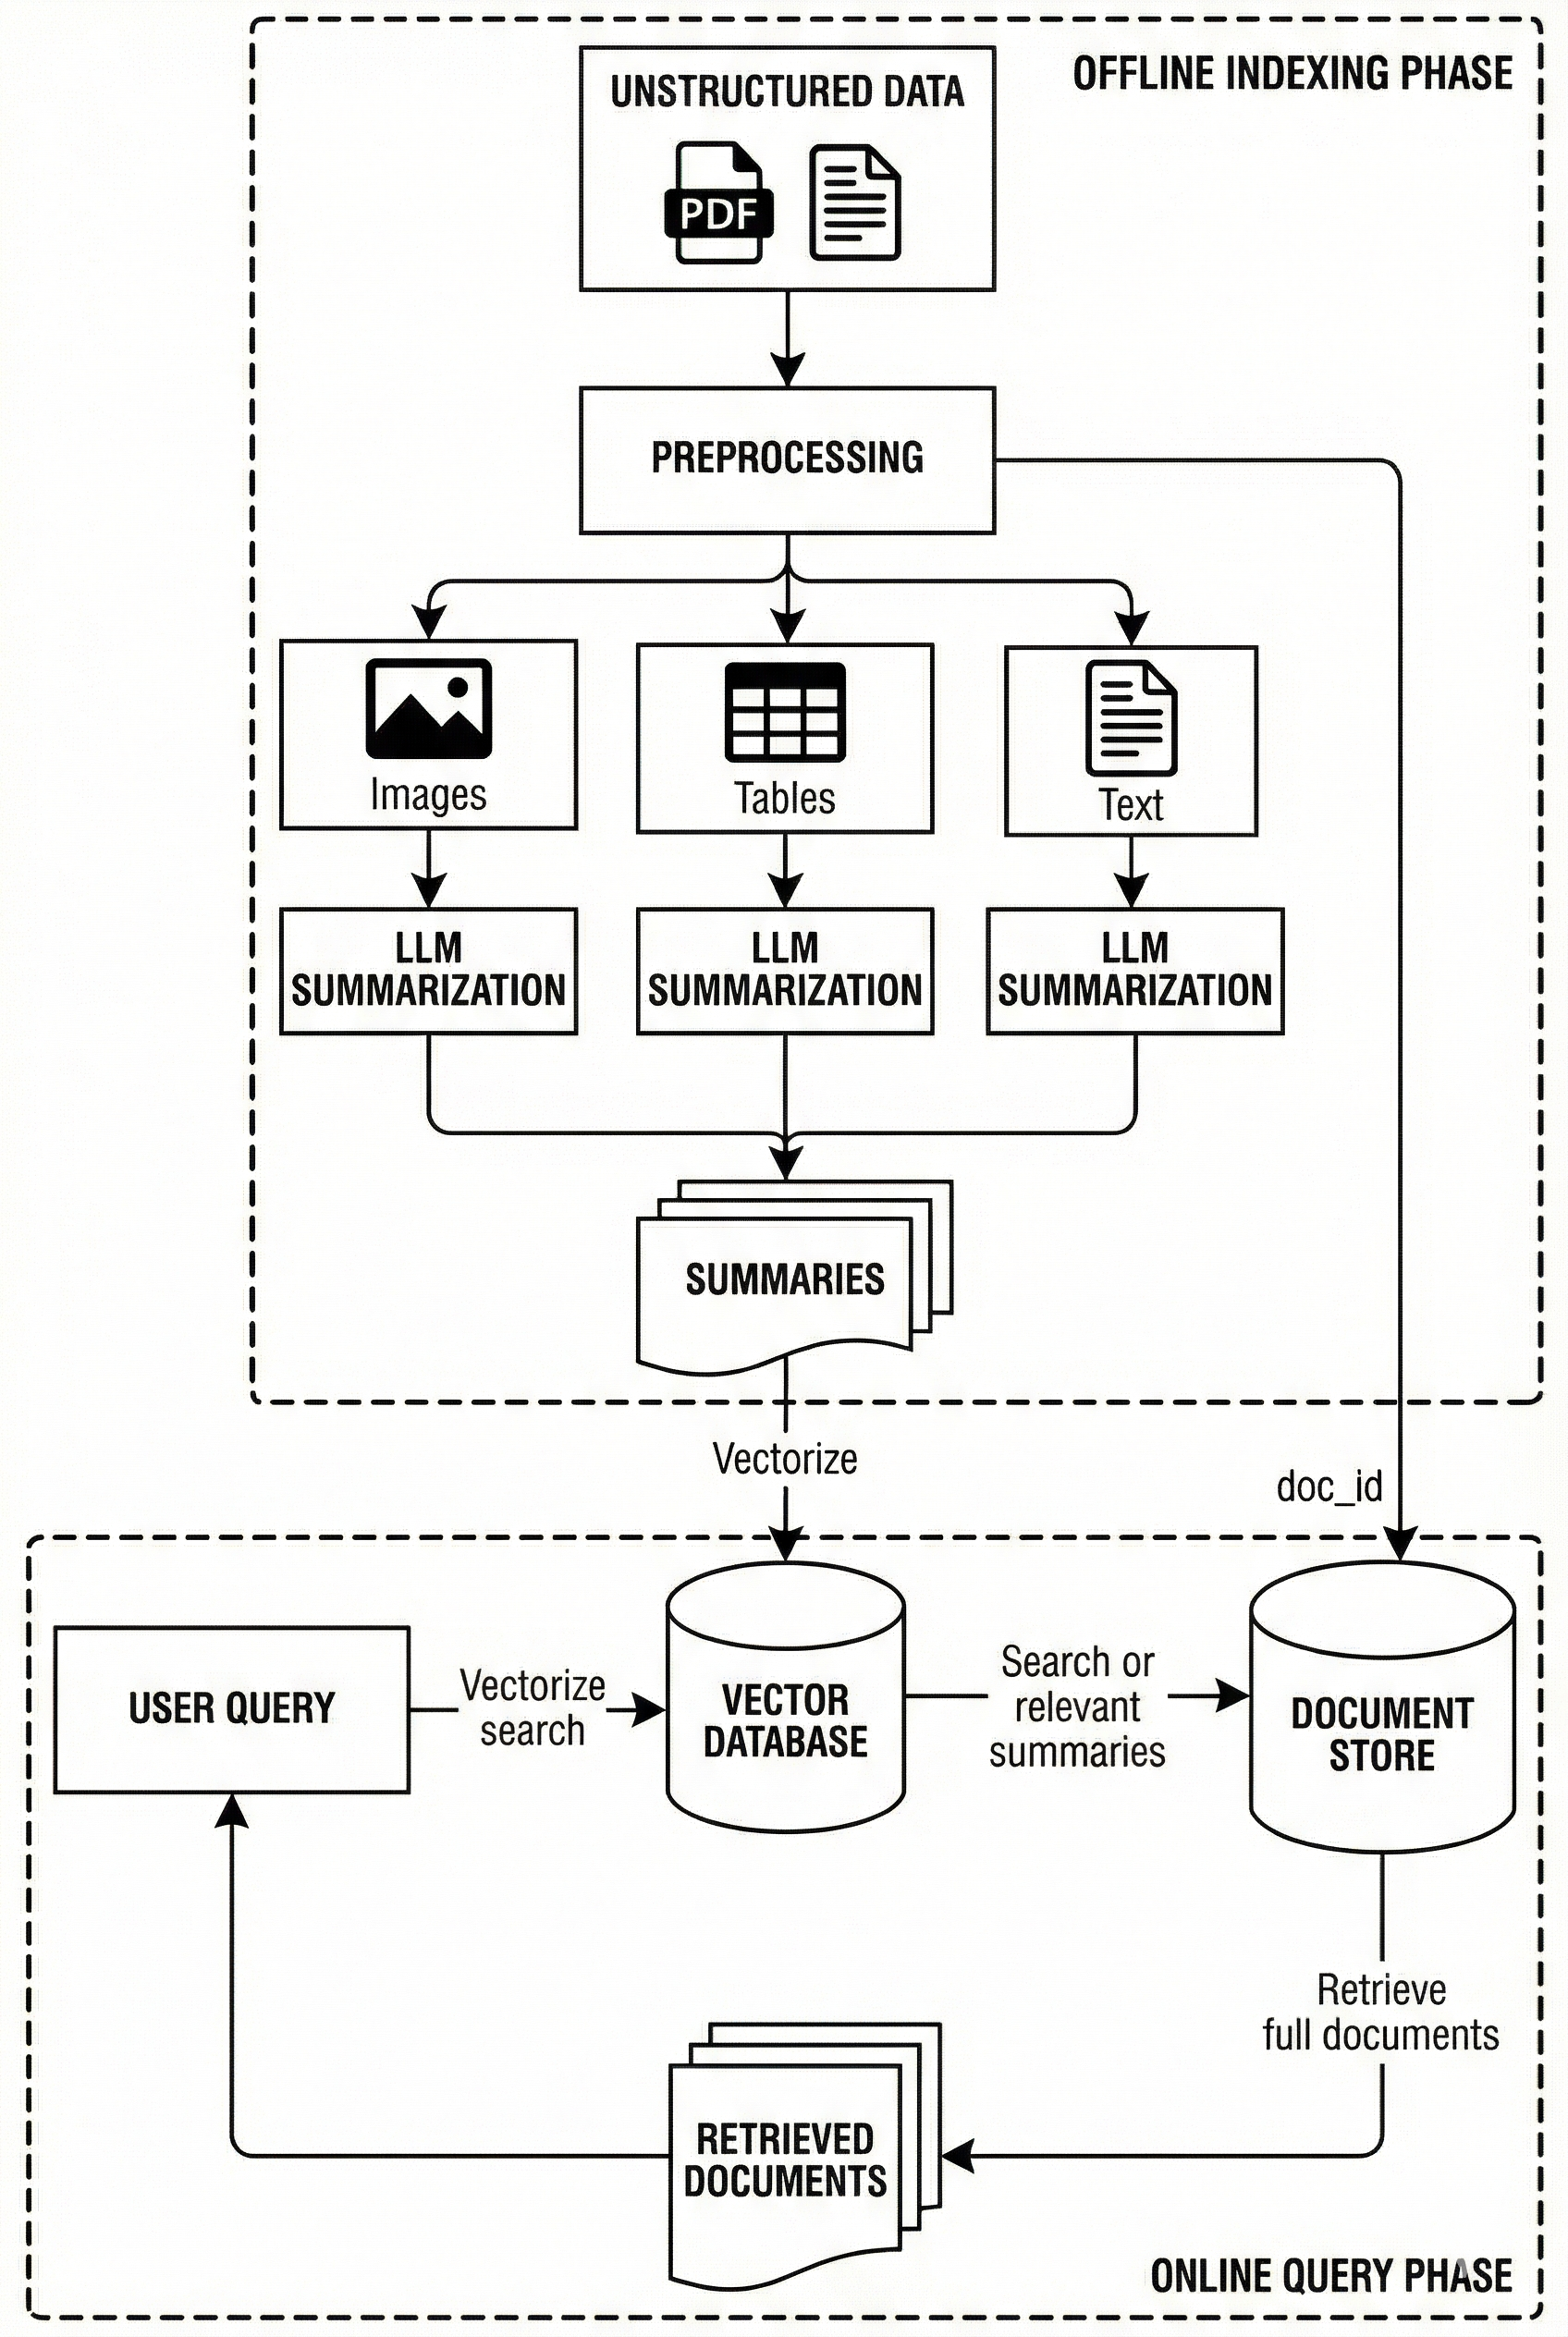
\includegraphics[width=0.6\textwidth]{figures/rag_pipeline_diagram.png}
    \caption{Advanced RAG Pipeline Architecture Diagram}
    \label{fig:rag_pipeline_diagram}
\end{figure}

The Pipeline is organized into two phases: \textbf{Indexing Phase} (offline, runs once when new documents arrive) and \textbf{Query Phase} (online, each time a user asks a question).

\subsection{Indexing Phase: Restructuring Knowledge}

\subsubsection{Preserving Structure with UnstructuredIO and Table Transformer}

To solve the problem of losing table structure during parsing, we use UnstructuredIO \parencite{unstructured_io}---a powerful library for Document Layout Analysis. Instead of PyPDF which only extracts raw text, UnstructuredIO uses computer vision to detect regions in PDFs: Text blocks, Table regions, and Image regions. Specifically, for tables, UnstructuredIO preserves the 2D structure by converting to HTML.

We use the \texttt{hi\_res} strategy of UnstructuredIO. With this strategy, UnstructuredIO treats each document page as an image and passes it through Object Detection models like YoloX or Detectron2 to classify regions in the page as Title, Text, List, Table, Image and predict ``bounding boxes'' around each component. Particularly, for regions marked as ``Table'', UnstructuredIO not only extracts text but also needs to understand the row/column structure using Table Transformer (TATR) \parencite{smock2021pubtables}. The process works as: 
\begin{enumerate}
    \item \textbf{Table Detection}: Identify table positions. 
    \item \textbf{Table Structure Recognition}: Recognize lines (cells), merged cells, and classify headers vs. body. 
    \item \textbf{HTML Mapping}: Finally, map these coordinates to \texttt{<table>} tags for easy LLM processing.
\end{enumerate}

Figure \ref{fig:unstructuredio_table_detection} and the HTML output below illustrates an example of table detection and extraction using UnstructuredIO.

\begin{figure}[H]
    \centering
    \includegraphics[width=0.8\textwidth]{figures/unstructuredio_table_detection.png}
    \caption{Table extraction process using UnstructuredIO and TATR}
    \label{fig:unstructuredio_table_detection}
\end{figure}

\begin{htmlcode}
  <table>
      <thead>
          <tr>
              <th>Sous modules (en k€)</th>
              <th>SCR 2024</th>
              <th>SCR 2023</th>
              <th>Evolution</th>
          </tr>
      </thead>
      <tbody>
          <tr>
              <td>Type 1</td>
              <td>2 692</td>
              <td>2 487</td>
              <td>8%</td>
          </tr>
          <tr>
              <td>Type 2</td>
              <td>28 377</td>
              <td>36 221</td>
              <td>-22%</td>
          </tr>
          <tr>
              <td>Effet de diversification</td>
              <td>-621</td>
              <td>-586</td>
              <td>6%</td>
          </tr>
          <tr>
              <td>Risque de défaut</td>
              <td>30 448</td>
              <td>38 121</td>
              <td>-20%</td>
          </tr>
      </tbody>
  </table>
\end{htmlcode}

Using the same table as in the PyPDF test above, we now preserve the table structure in HTML. This structure will be fed to the LLM. Using HTML as an intermediate format for tables is optimal because modern LLMs (like Gemma-3) are trained on large amounts of web data, giving them the ability to ``understand'' and ``reason'' on \texttt{<table>} structures much better than plain text.

\subsubsection{Semantic Bridge: Summarization Mechanism for Multimodal Data}

To bridge the semantic gap between user questions and dry numbers in tables/images, we deploy a Summarization layer. Current embedding models often struggle with:

\begin{itemize}
  \item \textbf{Tables}: Tables that are too large or contain pure numerical data (e.g., ``2024: 210,294'') often lack contextual keywords (like ``revenue'', ``growth''), making retrieval inaccurate.
  \item \textbf{Images}: Traditional embedding models cannot ``read'' content directly from images.
\end{itemize}

\textbf{Solution}: Use LLM to create summaries for each data chunk, serving as a ``semantic bridge'' to increase content identification efficiency.

We use Gemma-3-12b-it to analyze complex numerical tables in chunks. The LLM will interpret numbers into meaningful text (e.g., ``The table shows revenue for 2024 reached 210,294 k€, up 6\%''). This helps the chunk embedding match accurately with user's descriptive queries. For chunks containing images, since Gemma-3-12b-it is a Multimodal LM capable of converting visual information to text descriptions. This process helps the embedding model ``understand'' image content through the auxiliary summary layer.

For the table in the image \ref{fig:unstructuredio_table_detection}, the summary is generated as follows:

\begin{center}
    \fbox{
    \begin{minipage}{0.95\textwidth}
        \footnotesize
        \textbf{Summary:} "Le tableau détaille l'évolution du Solvency Capital Requirement (SCR) pour différents sous-modules entre 2023 et 2024, avec les montants exprimés en milliers d'euros (k€) et l'évolution en pourcentage. 

        Pour le sous-module << Type 1 >>, le SCR est passé de 2 487 k€ en 2023 à 2 692 k€ en 2024, affichant une évolution de 8\%. Le sous-module << Type 2 >> a vu son SCR passer de 36 221 k€ en 2023 à 28 377 k€ en 2024, avec une évolution indiquée de -22\%. 

        L'<< Effet de diversification >> a évolué de -586 k€ en 2023 à 621 k€ en 2024, soit une évolution de 6\%. Enfin, le << Risque de défaut >> a diminué, passant de 38 121 k€ en 2023 à 30 448 k€ en 2024, l'évolution diminue de -20\%."
    \end{minipage}
    }
\end{center}

This summary becomes a "semantic bridge": when a user asks about "revenue in 2024," the question's embedding will have a high similarity to the summary (containing "coffee shop" and "2024"). This enriches the information for the chunk, ensuring the highest possible similarity between the query vector and the document content, even if the original data does not contain the keywords in the question.
\subsubsection{Parent-Child Indexing Strategy}

After the summary generation step, each chunk now has two parts: raw content and its summary. The summary will be stored in the vector store for retrieval. However, if we use this summary as context for the LLM, the LLM will lack the necessary information to answer in detail. Short summaries help more accurate retrieval (less noise), but LLMs need complete raw content (including HTML tables) to generate detailed answers. Therefore, we apply \textbf{Parent-Child Indexing Strategy}. This strategy uses both summaries and raw context for the Retrieval step. The process can be described as follows:
\begin{enumerate}
    \item Index summary embeddings into ChromaDB/Qdrant with linked \texttt{doc\_id}.
    \item Store raw content (text, HTML tables, base64 images) in InMemoryStore.
    \item During retrieval, find similar summaries, then fetch corresponding raw content by \texttt{doc\_id}.
\end{enumerate}

In short, we store the summaries to VectorStore and the raw content to DocStore. Then, summaries are responsible for locating relevant chunks. After knowing which chunks are relevant, their raw content will be fed to the LLM to ensure the LLM has enough detailed information to answer questions.

\subsubsection{Multilingual Embedding Model}

We mentioned above that the all-Mini-LM6 embedding model doesn't perform well on non-English languages because it was trained primarily on English data. Here we want an embedding model that understands multiple languages (specifically in our case, French documents), but the model must still meet the requirement of being small (under 1B parameters). Based on the MTEB leaderboard, we selected \texttt{intfloat/multilingual-e5-large-instruct}.

\begin{figure}[H]
    \centering
    \includegraphics[width=0.8\textwidth]{figures/mteb_multilingual_comparison.png}
    \caption{Comparison of the performance of embedding models on MTEB Multilingual}
    \label{fig:mteb_multilingual}
\end{figure}

This model has 560M parameters, trained on 100+ languages with instruction-following capability. At the time of building the pipeline, this was the best \footnote{Currently there are newer models like \texttt{Qwen3-embeddings-0.6B} that could be used as alternatives to optimize the pipeline} retriever model under 1B parameters for multilingual data.

\subsection{Query Phase: Multi-modal Knowledge Query and Synthesis Mechanism}

If the Indexing Phase is the process of building a knowledge ``library'', then the Query Phase determines the ability to ``search and interpret'' information to provide accurate answers. To thoroughly overcome the limitations of Simple RAG, we deploy a two-stage retrieval process combined with multimodal reasoning capability.

\subsubsection{Hybrid Search: Combining Semantic and Keyword}

As analyzed in section \ref{sec:exact_code_matching_issue}, queries containing identifier codes (like CCAM code "HAFA008") often fail in Vector space (Dense Search) due to the distributed nature of embeddings. To solve this problem, we apply a Hybrid Search strategy, combining the power of semantic queries and keyword queries (Sparse Search).



\textbf{Coordination mechanism}: We use the BM25 (Best Matching 25) algorithm to exactly capture specific keywords (exact match) and Dense Search with the \texttt{multilingual-e5-large} model to understand context. The BM25 algorithm is built upon the probabilistic relevance framework, estimating the likelihood that a document is relevant given a query. For a query $Q$ containing terms $q_1, q_2, \ldots, q_n$, the relevance score of document $D$ is computed as:

\[
\text{BM25}(D, Q) = \sum_{i=1}^{n} \text{IDF}(q_i) \cdot \frac{f(q_i, D) \cdot (k_1 + 1)}{f(q_i, D) + k_1 \cdot \left(1 - b + b \cdot \frac{|D|}{\text{avgdl}}\right)}
\]

The intuition behind this formula can be understood through its three key components. The IDF (Inverse Document Frequency) term, defined as $\text{IDF}(q_i) = \log \frac{N - n(q_i) + 0.5}{n(q_i) + 0.5}$, assigns higher weights to rare terms that appear in fewer documents, reflecting their discriminative power. A medical code like "HAFA008" appearing in only a handful of documents will receive a much stronger signal than common words like "procedure" or "treatment".

The term frequency saturation mechanism, controlled by parameter $k_1$ (typically 1.2--2.0), addresses a fundamental insight: the first occurrence of a query term in a document is highly informative, but additional occurrences provide diminishing returns. Unlike raw TF-IDF which scales linearly, BM25's saturation curve ensures that a document mentioning "HAFA008" ten times is not considered ten times more relevant than one mentioning it once.

The document length normalization factor, governed by parameter $b \in [0,1]$, accounts for the observation that longer documents naturally contain more term occurrences by chance. When $b=1$, full normalization is applied relative to the average document length $\text{avgdl}$; when $b=0$, no length penalty is imposed. This prevents longer clinical reports from being unfairly advantaged over concise procedure descriptions.

\textbf{Dense Retrieval with Embeddings.} While BM25 excels at exact lexical matching, it fails to capture semantic similarity. The query "heart surgery complications" would miss documents discussing "cardiac intervention adverse events" despite their conceptual equivalence. Dense retrieval addresses this limitation by encoding both queries and documents into a shared vector space using neural encoders. We employ the \texttt{multilingual-e5-large} model, which maps text to 1024-dimensional embeddings where semantic similarity corresponds to geometric proximity, measured via cosine similarity or dot product.

\textbf{The Fusion Challenge.} Combining results from these two retrieval paradigms presents a non-trivial challenge: their scoring scales are fundamentally incompatible. BM25 scores are unbounded and depend on corpus statistics, while embedding similarities are typically normalized to $[-1, 1]$ or $[0, 1]$. Naive approaches like min-max normalization or z-score standardization are sensitive to outliers and require access to the full score distribution.

\textbf{Reciprocal Rank Fusion.} RRF elegantly sidesteps the score calibration problem by operating solely on rank positions. Given a document $d$ retrieved by multiple systems, its fused score is:

\[
\text{RRF}(d) = \sum_{r \in R} \frac{1}{k + \text{rank}_r(d)}
\]

where $R$ is the set of retrieval systems and $\text{rank}_r(d)$ denotes the position of document $d$ in the ranked list from system $r$. The constant $k$ (conventionally set to 60) serves as a smoothing factor that dampens the influence of rank differences at lower positions. Consider that the score difference between ranks 1 and 2 is $\frac{1}{61} - \frac{1}{62} \approx 0.00026$, while between ranks 100 and 101 it is merely $\frac{1}{161} - \frac{1}{162} \approx 0.000038$---nearly an order of magnitude smaller. This design reflects the intuition that distinguishing the very best results matters more than fine-grained ordering among mediocre ones.

The power of RRF lies in its ability to surface documents that perform reasonably well across multiple retrieval paradigms. A document ranked 5th by BM25 and 8th by dense retrieval (RRF score $\approx 0.030$) will outrank one that is 1st by BM25 but 50th by dense retrieval (RRF score $\approx 0.025$). This consensus-based ranking proves particularly effective for medical queries where both exact code matching and semantic understanding are essential.


\subsubsection{Cross-Encoder Reranking: Solving the ``Lost in the Middle'' Phenomenon}

Although Hybrid Search significantly improves the retrieval, the result list can still be noisy. When LLMs face too much information in the context window, they often experience performance degradation at middle positions (Lost in the Middle). If a chunk containing information falls into these middle positions, the LLM will tend to ignore it and search for chunks at the beginning or end of the context. We solve this problem with a Reranker layer using \textbf{Cross-Encoder architecture}.

\textbf{Architectural difference}: Unlike Bi-Encoder (e.g. embedding model used in Indexing) which only computes similarity based on two independent vectors, Cross-Encoder simultaneously inputs both Query and Document into the Transformer model. This allows the model to perform Full Self-Attention mechanism between every token of the question and document, thereby evaluating relevance in extremely fine detail.

\textbf{Optimization strategy}: Due to the high computational cost of Cross-Encoder, we only perform re-ranking on the top-10 candidates from the Hybrid Search step. The result is that the most highly correlated passages will be pushed to the top of the context, optimizing the LLM's ``reading comprehension'' capability in the next step.

\subsubsection{Multimodal Generation: Synthesizing Knowledge from Text, Tables and Images}

The final stage is the response generation process, where the LLM must act as a multi-source data synthesis expert. Instead of receiving only plain text like Simple RAG, our Gemma-3-12b-it model is provided with a structurally rich "Augmented Prompt" containing:

\begin{itemize}
  \item \textbf{2D Structure}: Financial tables are passed in original HTML format, helping the LLM maintain alignment between columns (fiscal years) and rows (revenue metrics), completely eliminating errors from reading wrong numbers due to text flattening.
  \item \textbf{Visual Information}: For chunks containing charts or medical illustration images, the model receives image data directly (Base64) along with summaries created in the Indexing step.
  \item \textbf{Guardrails}: The prompt is designed with Chain-of-Thought (CoT) technique, requiring the model to directly cite data sources from context to minimize hallucination.
\end{itemize}


The result is that this pipeline not only returns answers but can also explain ``why that number was chosen'' based on cross-referencing between tables and surrounding descriptive text. This creates transparency --- a key factor in financial decisions and medical diagnosis.

\section{Experimental Evaluation}

To demonstrate the effectiveness of the proposed Advanced RAG architecture, we conduct quantitative evaluation on two real-world datasets from partners, while also performing Ablation Study to determine the contribution value of each technical component.

\subsection{Experimental Setup}

\subsubsection{Test Datasets (Testbeds)}

\textbf{GPM Test Set}: Comprises 25 question-answer (Q\&A) pairs manually labeled by financial experts from AGMF documents. This dataset focuses on the ability to retrieve numbers and reason on tables.

\textbf{CCAM Test Set}: Comprises 10 complex clinical consultation scenarios. Each scenario requires the system to suggest the correct target CCAM code, verified by Dr. Besnier.

\subsubsection{Evaluation Metrics System}

We employ the RAGAS (Retrieval-Augmented Generation Assessment) evaluation framework combined with the LLM-as-a-Judge methodology to ensure objective and reproducible assessment of our RAG pipeline.

\textbf{LLM Judge Selection}: To mitigate potential bias from relying on a single evaluator model, we utilize two open-weight LLMs as judges: \textbf{Gemma-3-12B-Instruct} and \textbf{Mistral-Small-24B-Instruct-2501}.

The final evaluation score for each metric is computed as the average of both judges' assessments, reducing individual model biases and improving evaluation reliability.

\textbf{Retrieval Quality Metrics}:
\begin{itemize}
    \item \textbf{Context Precision}: Measures the proportion of relevant chunks among all retrieved chunks, evaluating the Retriever's ability to prioritize useful information at the top of the ranked list. Formally defined as:
    \begin{equation}
        \text{Context Precision} = \frac{1}{K} \sum_{k=1}^{K} \frac{\text{Relevant chunks in top } k}{k}
    \end{equation}
\end{itemize}

\textbf{Generation Quality Metrics}:
\begin{itemize}
    \item \textbf{Faithfulness}: Quantifies the factual consistency between the generated answer and the retrieved context. Each claim in the answer is verified against the context to compute:
    \begin{equation}
        \text{Faithfulness} = \frac{|\text{Claims supported by context}|}{|\text{Total claims in answer}|}
    \end{equation}
    This metric is critical for controlling hallucination in domain-specific applications.
    
    \item \textbf{Answer Relevancy}: Evaluates the pertinence and completeness of the generated answer with respect to the user query. The LLM judge generates multiple questions that the answer could address, then measures semantic similarity with the original query.
    
    \item \textbf{Answer Correctness}: Performs semantic comparison between the system-generated answer and the ground-truth reference answer, yielding a score on a continuous scale from 0 to 1. 
    
    % This metric combines both factual overlap and semantic similarity:
    % \begin{equation}
    %     \text{Answer Correctness} = \alpha \cdot F_1^{\text{factual}} + (1-\alpha) \cdot \text{Semantic Similarity}
    % \end{equation}
    % where $\alpha = 0.5$ balances factual accuracy and semantic equivalence.
\end{itemize}

\textbf{Domain-Specific Metrics}:
\begin{itemize}
    \item \textbf{Code Hit Rate@k (For CCAM)}: Measures the proportion of test cases where the correct CCAM code appears within the top $k$ retrieval results:
    \begin{equation}
        \text{Hit Rate@}k = \frac{1}{N} \sum_{i=1}^{N} \mathbb{1}[\text{correct code}_i \in \text{top-}k \text{ results}_i]
    \end{equation}
    We report Hit Rate@5 and @20 to evaluate retrieval precision at different cut-off points.
\end{itemize}

All metrics are computed independently by both LLM judges, and we report the mean score to validate evaluation consistency.

\subsection{Comparison Results: Simple RAG vs. Advanced RAG}

Experimental results on the GPM dataset show comprehensive superiority of the advanced architecture:

\begin{table}[H]
    \centering
    \caption{Results on GPM Test Set (25 questions)}
    \begin{tabular}{|l|c|c|c|c|}
        \hline
        \textbf{Pipeline} & \textbf{Correctness} & \textbf{Relevancy} & \textbf{Faithfulness} & \textbf{Context Precision} \\
        \hline
        Simple RAG & 0.648 & 0.788 & 0.732 & 0.654 \\
        \hline
        Advanced RAG & \textbf{0.976} & \textbf{0.972} & \textbf{0.94} & \textbf{0.96} \\
        \hline
        \textit{Improvement} & \textit{+32.8\%} & \textit{+18.4\%} & \textit{+20.8\%} & \textit{+30.6\%} \\
        \hline
    \end{tabular}
\end{table}

The strongest increases are in Context Precision (+30.6\%) and Answer Correctness (+32.8\%). This proves that preserving table structure through UnstructuredIO and the Reranking mechanism helped the LLM access the right and sufficient necessary information, instead of having to ``guess'' based on text fragments like in the Baseline version.

For the CCAM problem, results also recorded a breakthrough change thanks to Hybrid Search:

\begin{table}[H]
    \centering
    \caption{Results on CCAM Test Set (10 scenarios)}
    \begin{tabular}{|l|c|c|}
        \hline
        \textbf{Pipeline} & \textbf{Code Hit Rate@5} & \textbf{Code Hit Rate@20} \\
        \hline
        Simple RAG & 0.4 & 0.6 \\
        \hline
        Advanced RAG & \textbf{0.8} & \textbf{0.9} \\
        \hline
        \textit{Improvement} & \textit{+40\%} & \textit{+30\%} \\
        \hline
    \end{tabular}
\end{table}

Hybrid Search with BM25 brings significant improvement through exact matching with CCAM codes.

\section{Ablation Study: Contribution of Each Component}

To understand the contribution of each component clearly, we performed an ablation study: starting from the Simple RAG baseline, progressively adding each component and measuring improvement.

\begin{table}[H]
    \centering
    \caption{Ablation Study on GPM Test Set}
    \begin{tabular}{|l|c|c|c|}
        \hline
        \textbf{Configuration} & \textbf{Precision} & \textbf{$\Delta$ vs Baseline} & \textbf{Cumulative $\Delta$} \\
        \hline
        Baseline (Simple RAG) & 0.648 & --- & --- \\
        \hline
        + UnstructuredIO Parsing & 0.762 & +11.4\% & +11.4\% \\
        \hline
        + Summarization & 0.818 & +5.6\% & +17.0\% \\
        \hline
        + Multilingual E5 Embedding & 0.875 & +5.7\% & +22.7\% \\
        \hline
        + Hybrid Search & 0.92 & +4.5\% & +27.2\% \\
        \hline
        + Reranking & \textbf{0.976} & +5.6\% & \textbf{+32.8\%} \\
        \hline
    \end{tabular}
\end{table}

\subsection{Detailed Analysis of Each Component}

\textbf{UnstructuredIO Parsing (+11.4\%)}: This is the most important contributing component. Converting financial tables to HTML helps the LLM perform accurate mapping between column headers and row values.

\textbf{Summarization \& E5 (+11.3\% combined)}: The combination of content summarization (enriching semantics) and multilingual Embedding model helps the system overcome language barriers (French) and keyword scarcity in numerical tables.

\textbf{Hybrid Search \& Reranking (+10.1\% combined)}: These two components act as a ``fine filter''. Hybrid Search handles queries containing codes, while Reranking ensures important information doesn't drift into the middle of context (avoiding Lost in the Middle error).

\section{Discussion and Conclusions}

\subsection{Contributions}

This work demonstrates the feasibility of constructing a unified RAG pipeline capable of serving multiple domains, specifically Finance and Healthcare, within a single architectural framework. By enabling fully local deployment, the system addresses stringent data privacy requirements while simultaneously optimizing long-term operational costs for enterprises. The empirical results validate the effectiveness of our three-pillar approach—Structure Preservation through advanced parsing, Semantic Enrichment via multimodal summarization, and Multi-layer Retrieval combining Hybrid Search with Cross-Encoder reranking—yielding a 32.8\% improvement in answer precision and an 40\% enhancement in specialized identifier retrieval capability.

\subsection{Limitations and Future Directions}

Despite these promising outcomes, several limitations warrant consideration. The integration of Cross-Encoder reranking introduces additional latency of approximately 3-5 seconds per query, while multimodal summarization further extends input processing time. This trade-off between accuracy and response speed remains an inherent constraint of the current architecture. Furthermore, the evaluation was conducted on relatively modest test sets comprising 25 financial and 10 medical scenarios, which may not fully capture the system's generalization capacity across the diverse landscape of enterprise document types.

To address these challenges, future research will explore three primary directions. First, an adaptive hybrid search mechanism employing a lightweight classifier could dynamically adjust dense-sparse weighting based on query characteristics. Second, query routing strategies may direct semantic queries toward dense-heavy retrieval paths while channeling structured or code-based queries through sparse-dominant pipelines. Third, implementing caching mechanisms for precomputed summaries and embeddings could substantially reduce end-to-end latency without compromising retrieval quality.

\subsection{Conclusion}

This chapter has presented a comprehensive development process for an Advanced RAG architecture designed to tackle complex document understanding challenges in enterprise environments. Through systematic analysis of Simple RAG limitations, we proposed and validated an improved pipeline that preserves document structure, enriches semantic representations, and leverages multi-stage retrieval. The experimental findings not only fulfill the practical requirements of Torus AI's industry partners but also contribute a replicable framework to the broader RAG research community working with multimodal enterprise data.Claude is AI and can make mistakes. Please double-check responses.

%%------------------------------- CHAPTER 4: FINE-TUNING ------------------------------------

\chapter{Fine-tuning Small Language Models for Specialized Tasks: The Tarot Reader Case}
\label{chap:finetuning_slm_tarot}

Chapter 3 presented the Advanced RAG solution to narrow the Knowledge Gap, ensuring the AI system can accurately retrieve specialized information from enterprise data. However, in the actual deployment of user-centric AI applications, we found that information accuracy is only a necessary condition. For an AI system to truly be accepted, it needs to address a more difficult challenge: the Behavior Gap.

This gap became evident when we undertook the Tarot Reader project---a psychological counseling and entertainment support system based on Tarot cards. Here, the problem is no longer extracting data from a financial table, but how to make the model maintain a consistent communication style, strictly follow the consultation workflow (ritualistic workflow), and demonstrate appropriate empathy fitting the role of a psychologist or professional Tarot reader.

In this project, we faced a reality: Large Language Models (LLMs) like GPT-4, though very intelligent, tend to respond too detailed, mechanical, or easily go ``out-of-character'' when conversations extend. Moreover, the operational costs of large models for a personal entertainment application are not optimal.

Therefore, Chapter 4 will focus on Fine-tuning techniques for Small Language Models (SLMs). We aim to prove that: A model with only 0.5B to 1.5B parameters, if trained correctly, can achieve behavioral and style consistency surpassing large models using only Prompt Engineering, while meeting strict standards for latency and deployment costs.

\section{Problem Analysis: Why is Prompt Engineering Not Enough?}

\subsection{Limitations of In-Context Learning for Behavioral Tasks}

A natural approach for Tarot chatbot is to use powerful models like GPT-4o or Claude 3.5 with carefully designed system prompts. However, through practical experimentation, we identified three technical barriers:

\begin{itemize}
  \item \textbf{Attention Dilution}: Although modern models support large context windows (like 128K tokens of GPT-4), empirical research on the ``Lost in the Middle'' phenomenon indicates that model performance significantly degrades when important guiding information is buried in too long a context. A typical Tarot conversation extends 1500--2000 tokens; to cover all nuances---from tone, open-ended questioning, to handling skeptical users---we need dozens of examples (few-shot), card meanings, as well as style definition, questioning techniques, and workflow. Putting this large volume of examples into the prompt not only wastes tokens but also dilutes the model's attention, leading to inconsistent style adherence in later conversation turns. Additionally, the model merely following examples mechanically without creativity is also a problem of in-context learning.

  \item \textbf{Operational cost limitations}: Table \ref{tab:cost-comparison} compares costs between options. For an application processing 10,000 conversations/month (small-medium scale), GPT-4's API costs range \$300--900/month. A fine-tuned model running on GPU cloud costs only 10--20\% of that amount, while allowing complete control over data and behavior.

  \begin{table}[H]
      \centering
      \caption{Operational cost comparison. *Assuming 10K conversations × 3K tokens/conversation. **Amortized GPU cost.}
      \begin{tabular}{|l|c|c|}
          \hline
          \textbf{Option} & \textbf{Cost/1K tokens} & \textbf{Cost/month*} \\
          \hline
          GPT-4-turbo API & \$0.01--0.03 & \$300--900 \\
          Claude 3 Sonnet API & \$0.003--0.015 & \$90--450 \\
          Qwen-1.5B Fine-tuned (T4) & \$0.0005** & \$50--100 \\
          Qwen-0.5B Fine-tuned (Edge) & \$0.0001** & \$10--30  \\
          \hline
      \end{tabular}
      \label{tab:cost-comparison}
  \end{table}

  \item \textbf{Latency limitations}: Cloud APIs typically have 500ms--2s latency for the first token, creating a ``waiting'' feeling unsuitable for real-time consultation experience. Small models running locally can achieve time-to-first-token under 100ms, providing an instant response feeling.

\end{itemize}

\subsection{Specifics of the Tarot Reader Task}

Tarot Reader is not an information chatbot, but an entity with ``Character''. This task requires tight integration of three information layers:

\begin{itemize}
  \item \textbf{Knowledge Layer}: Meanings of 78 cards in both upright and reversed states.

  \item \textbf{Operational Layer}: Strictly following workflow: Greeting → Exploring issue → Inviting to draw cards → Interpreting each card → Synthesizing message.

  \item \textbf{Emotional Layer}: Using empathetic language, asking open-ended questions instead of rigid statements.
\end{itemize}

\subsection{Research Questions}

Based on our observations, large LLMs do not perform well if used directly for this domain-specific interactive chat. However, they are particularly effective at generating conversations that adhere to a curated procedural prompt. Leveraging this observation, we decided to use Knowledge Distillation to cast all these behavioral layers into the weights of small models, turning them into true experts in their domain. We set two main research questions:

\begin{itemize}
    \item \textbf{RQ1}: Can fine-tuned small models ($\leq$ 3B parameters) achieve behavioral consistency equivalent to or better than large LLMs with prompt engineering?
    \item \textbf{RQ2}: Is LoRA sufficient to learn behavioral patterns or is full fine-tuning needed?
\end{itemize}

\section{Knowledge Distillation Pipeline}

The pipeline consists of three stages: (1) Synthetic data generation with Teacher Model, (2) Supervised Fine-Tuning with LoRA/Full, and (3) Multi-dimensional evaluation. Figure 


\begin{figure}[H]
    \centering
    \fbox{\parbox{0.95\textwidth}{\centering
        \begin{tabular}{ccccc}
        \fbox{\parbox{2.5cm}{\centering \small Teacher Model\\(GPT-4o, Qwen-Plus)}} & 
        $\xrightarrow{\text{generate}}$ & 
        \fbox{\parbox{2.5cm}{\centering \small Synthetic\\Conversations}} & 
        $\xrightarrow{\text{filter}}$ & 
        \fbox{\parbox{2.5cm}{\centering \small Training\\Dataset}} \\
        & & & & $\downarrow$ \\
        \fbox{\parbox{2.5cm}{\centering \small LLM Judge +\\Human Eval}} & 
        $\xleftarrow{\text{evaluate}}$ & 
        \fbox{\parbox{2.5cm}{\centering \small Fine-tuned\\Model}} & 
        $\xleftarrow{\text{train}}$ & 
        \fbox{\parbox{2.5cm}{\centering \small Student Model\\+ LoRA}}
        \end{tabular}
    }}
    \caption{Pipeline Knowledge Distillation for Tarot Readers. The Teacher Model generates sample data, the Student Model learns from this data, and the results are evaluated by an LLM Judge and human evaluators.}
    \label{fig:finetuning-pipeline}
\end{figure}



\subsection{Synthetic Data Generation: Distillation at the Behavioral Level}

\subsubsection{Objectives and Data Format}

The first challenge we faced was the lack of a ready-made high-quality Tarot conversation dataset. Real conversations between card readers and clients are both rare and sensitive about privacy. Our solution is to apply Knowledge Distillation at a different level than traditional approaches: instead of distilling logits or hidden states, we distill \textit{behavioral patterns}---the behavior, tone, and working process of a Tarot expert.

Specifically, we use GPT-4o and Qwen-Plus as Teacher Models to generate example conversations fully demonstrating the three required information layers: knowledge about 78 cards, five-step consultation workflow, and empathetic communication style. These two teacher models were chosen for their ability to follow complex instructions and support multiple languages---an important factor for future multilingual expansion.

Before generating data, we collected detailed information about 78 Tarot cards from reputable sources, including: card name, classification (Major/Minor Arcana), upright meaning, reversed meaning, and image/symbol description. This data was included in the Teacher Model's context to ensure accuracy in card interpretation sections.

A typical Tarot conversation has the following structure:

\begin{tcolorbox}[breakable, colback=gray!5!white, colframe=gray!50!black, title=\textbf{Illustrative Example: Tarot Conversation}]
    \small
    \textbf{Querent:} Hi, I've been feeling stuck in my job lately. I'm not sure if I should stay or look for something new.

    \vspace{0.5em}
    \textbf{Chatbot:} Hey there! Career crossroads can be tricky, right? Before we dive into the cards, tell me a bit more --- what's making you feel stuck? Is it the work itself, the environment, or something else?

    \vspace{0.5em}
    \textbf{Querent:} It's mostly that I don't feel challenged anymore. The pay is good but I'm just going through the motions.

    \vspace{0.5em}
    \textbf{Chatbot:} Ah, the golden handcuffs situation! That's actually really common. So you're craving growth and meaning, not just a paycheck. Got it. Ready to see what the cards have to say? Focus on your question, take a deep breath, and pick three cards when you're ready.

    \vspace{0.5em}
    \textbf{Querent:} [Draws: The Tower (reversed), Eight of Cups, The Star]

    \vspace{0.5em}
    \textbf{Chatbot:} Ooh, interesting spread! Let's start with The Tower reversed in your first position. Usually The Tower upright is about sudden upheaval, but reversed? It's more like... you're \textit{avoiding} a necessary change. Maybe you already know things need to shake up, but you're holding on because it feels safer?
    
    The Eight of Cups in the middle --- this one's literally about walking away from something that no longer fulfills you. See how the figure is leaving those cups behind? That's you, being called to seek something more meaningful...
    
    \textit{[continues with card interpretations and synthesis]}
\end{tcolorbox}

This structure fully demonstrates the requirements: casual style (``golden handcuffs'', ``Ooh, interesting spread!''), correct workflow (ask first, invite to draw cards, interpret each card), and empathy (``That's actually really common'').

\subsubsection{Data Generation Strategy with Teacher Model}

We apply Knowledge Distillation at the \textit{behavioral patterns} level --- Teacher Model generates example conversations demonstrating the correct style and workflow, Student Model learns from these examples.

\textbf{Teacher Model}: Using GPT-4o and Qwen-Plus as Teachers for their ability to follow complex instructions and support multiple languages.

\textbf{Data generation process}:

\begin{enumerate}
    \item \textbf{Create initial questions}: Use LLM to generate a list of 100+ questions across 5 topics (career, relationships, health, personal growth, finance). Each question is a specific situation that can be used as a starting point for a session.
    
    \item \textbf{Define variations}: For each question, generate multiple conversations with variations:
    \begin{itemize}
        \item \textit{Length}: short (5--7 turns), moderate (8--10 turns), long (11--15 turns)
        \item \textit{Querent personality}: gentle, expressive, doubtful, skeptical, rude, rejective
        \item \textit{Card combination}: Random 3 cards from 78, 30\% probability for each card to be reversed
    \end{itemize}
    
    \item \textbf{Generate conversation}: Teacher Model receives system prompt, information about drawn cards, and querent persona to generate complete conversations.
\end{enumerate}

\subsubsection{Filtering and Quality Control}

After generating raw data, we apply a filtering process:

\begin{enumerate}
    \item \textbf{Automatic filtering}:
    \begin{itemize}
        \item Remove conversations too short ($<$ 5 turns) or too long ($>$ 15 turns)
        \item Remove conversations with high repetition (Jaccard similarity between consecutive turns $>$ 0.7)
    \end{itemize}
    
    \item \textbf{Results}: From 366 raw conversations for each teacher model Qwen Plus and GPT-4o, we obtained 732 high-quality conversations ($\sim$585K tokens).

    \item \textbf{Human review}: 20\% of samples were read by annotators to evaluate naturalness and adherence to style guide. Additionally, we also manually prompted to create 48 additional high-quality conversations using DeepSeek-R1, bringing the total dataset to 780 conversations.
\end{enumerate}

\subsection{Model Selection and Training}

\subsubsection{Base Model Selection}

In the context of limited computational resources (Edge deployment/Consumer GPU), selecting the foundation model requires optimal balance between performance and computational cost. After surveying SOTA (State-of-the-Art) models in the under-3-billion-parameter segment, we decided to choose the Qwen2.5-Instruct model family (0.5B and 1.5B variants) based on two main reasons:

\begin{itemize}
  \item \textbf{Superior Performance-to-Parameter Ratio}: Experimental data on standard benchmarks (Table \ref{tab:model-comparison}) shows Qwen2.5-1.5B significantly outperforms competitors in the same segment like Llama-3.2-1B or Gemma-2-2.6B. Notably, MMLU score (general knowledge) reaches 60.9, approaching 7B models of previous generations. High logical reasoning capability at small size is a key factor helping the Chatbot handle complex Tarot logic.
  \begin{table}[H]
      \centering
      \caption{Performance comparison on standard benchmarks. Data extracted from Qwen2.5 Technical Report (2024).}
      \small
      \begin{tabular}{lcccc}
          \toprule
          \textbf{Model} & \textbf{Params} & \textbf{MMLU} & \textbf{GSM8K} & \textbf{MATH} \\
          \ & & (Knowledge) & (Reasoning) & (Hard Logic) \\
          \midrule
          Llama-3.2-1B-Instruct & 1.23B & 49.3 & 44.4 & 30.6 \\
          Gemma-2-2.6B-Base & 2.6B & 52.2 & 30.3 & 25.3 \\
          \textbf{Qwen2.5-0.5B-Instruct} & \textbf{0.49B} & 47.5 & \textbf{49.6} & \textbf{34.4} \\
          \textbf{Qwen2.5-1.5B-Instruct} & \textbf{1.54B} & \textbf{60.9} & \textbf{73.2} & \textbf{55.2} \\
          \bottomrule
      \end{tabular}
      \label{tab:model-comparison}
  \end{table}
  \item \textbf{Multilingual capability}: Unlike the Llama family focusing mainly on English and European languages, Qwen, a model from China, was trained on multilingual data with more than 29 languages. Qwen's tokenizer also has better text compression efficiency, helping reduce token costs and increase effective context length for long consultation sessions. 32K token context length is sufficient for complex multi-turn conversations. Additionally, Qwen's Apache 2.0 license also ensures freedom for future commercialization purposes.
\end{itemize}


\subsubsection{LoRA or Full Fine-tuning?}

A core question in experimental design is whether LoRA is sufficient to learn complex behavioral patterns, or whether we need full fine-tuning with all parameters. The theory of \textit{intrinsic dimensionality} suggests that adaptation tasks often lie in a low-dimensional subspace of the original parameter space --- LoRA with sufficiently high rank can capture this subspace without updating all weights.

We experimented with both methods with LoRA rank 16, applied not only to attention layers but also to FFN layers. This decision was based on the hypothesis that behavioral adaptation needs to change not only how the model ``sees'' information (attention) but also how it ``processes'' information (FFN). Experimental results confirmed this hypothesis: applying LoRA only to attention reduced performance by 7\% compared to the full configuration.

Regarding training configuration, we used effective batch size 8, learning rate 3e-5 with cosine scheduler, and especially applied \texttt{DataCollatorForCompletionOnlyLM} to only compute loss on the assistant response portion. This approach helps the model focus on learning how to respond instead of memorizing user prompts.

\subsection{Evaluation: Combining LLM Judge and Human Evaluation}

Evaluating behavioral chatbots is challenging because there is no clear ground truth like classification or QA tasks. A response can be correct in content but wrong in tone, or vice versa. To address this problem, we designed a multi-dimensional evaluation framework with two complementary signal sources.

The first source is LLM-as-a-Judge with two different evaluator models --- Gemma-3-12B-Instruct and Mistral-Small-24B-Instruct --- to reduce bias from a single judge. Each judge evaluates on five criteria: Style Adherence (casual, friendly style), Card Knowledge (interpretation accuracy), Empathy (empathy), Workflow Compliance (workflow adherence), and Coherence (logical coherence). Scores from two judges are averaged for more stable results.

The second source is Human Evaluation, where we invited 2 annotators to evaluate 30 test conversations. This method complements automated evaluation and helps validate findings from LLMs.

\section{Experimental Results}

\subsection{Training Process}

Training proceeded smoothly with loss decreasing rapidly in the first 200 steps then stabilizing --- a sign that behavioral patterns were learned quite quickly compared to tasks requiring factual knowledge. Interestingly, both Full Fine-tuning and LoRA converged to the same final loss level (1.12 vs 1.15 for Qwen-1.5B), but LoRA saved 15--20\% time and VRAM. The 3B model achieved the lowest loss (0.98) but training time was double that of 1.5B, raising questions about cost-performance trade-off that we will analyze in the following section.

\begin{table}[H]
  \centering
  \caption{Training results on NVIDIA T4 (16GB), 10 epochs}
    \begin{tabular}{|l|l|c|c|c|}
        \hline
        \textbf{Model} & \textbf{Method} & \textbf{Final Loss} & \textbf{Time} & \textbf{VRAM} \\
        \hline
        Qwen2.5-0.5B & Full FT & 1.35 & 3 min & 5.2 GB \\
        Qwen2.5-1.5B & Full FT & 1.18 & 9 min & 9.8 GB \\
        Qwen2.5-1.5B & LoRA r=16 & 1.15 & 62 min & 9.8 GB \\
        Qwen2.5-3B & LoRA r=16 & 0.98 & 2.1 hrs & 14.2 GB \\
        \hline
    \end{tabular}
    \label{tab:training-results}
\end{table}

\subsection{LLM-as-a-Judge Results}

Table \ref{tab:llm-judge-results} presents evaluation results from two LLM judges. These results show three important insights.

\begin{table}[H]
    \centering
    \caption{LLM-as-a-Judge Results. FT = Fine-tuned. Highlighted row: best overall model.}
    \small
    \begin{tabular}{|l|c|c|c|c|c|c|}
        \hline
        \textbf{Model} & \textbf{Style} & \textbf{Knowledge} & \textbf{Empathy} & \textbf{Workflow} & \textbf{Coherence} & \textbf{Avg} \\
        \hline
        \multicolumn{7}{|c|}{\textit{Judge: Gemma-3-12B-Instruct}} \\
        \hline
        Qwen-0.5B (base) & 0.42 & 0.65 & 0.48 & 0.35 & 0.72 & 0.52 \\
        Qwen-0.5B (FT) & 0.78 & 0.72 & 0.81 & 0.85 & 0.80 & 0.79 \\
        Qwen-1.5B (base) & 0.55 & 0.71 & 0.58 & 0.42 & 0.78 & 0.61 \\
        \rowcolor{gray!20}
        Qwen-1.5B (FT) & \textbf{0.88} & 0.85 & \textbf{0.89} & \textbf{0.92} & 0.88 & \textbf{0.88} \\
        Qwen-3B (FT) & 0.86 & \textbf{0.88} & 0.87 & 0.90 & \textbf{0.91} & 0.88 \\
        GPT-4 (prompt) & 0.82 & 0.90 & 0.85 & 0.75 & 0.92 & 0.85 \\
        \hline
        \multicolumn{7}{|c|}{\textit{Judge: Mistral-Small-24B-Instruct}} \\
        \hline
        Qwen-1.5B (base) & 0.52 & 0.68 & 0.55 & 0.40 & 0.75 & 0.58 \\
        \rowcolor{gray!20}
        Qwen-1.5B (FT) & \textbf{0.85} & 0.82 & \textbf{0.86} & \textbf{0.90} & 0.86 & \textbf{0.86} \\
        GPT-4 (prompt) & 0.80 & \textbf{0.88} & 0.82 & 0.72 & \textbf{0.90} & 0.82 \\
        \hline
    \end{tabular}
    \label{tab:llm-judge-results}
\end{table}

\textbf{Detailed Analysis}:

\begin{enumerate}
    \item \textbf{Fine-tuning improves comprehensively}: Qwen-1.5B increased from 0.55 to 0.88 (+33\%). The largest improvement is in Workflow Compliance (+50\%: 0.42 → 0.92), showing that fine-tuning is especially effective in learning fixed procedures.
    
    \item \textbf{Fine-tuned small models can outperform prompted large models on behavioral metrics}: Qwen-1.5B Fine-tuned achieved Style 0.88 compared to 0.82 of GPT-4, and Workflow 0.92 compared to only 0.75. GPT-4 has higher Knowledge (0.90 vs 0.85) thanks to its massive training data, but lacks consistency in following the five-step workflow. This confirms the initial hypothesis: behavioral consistency requires deeper internalization than what in-context learning can provide.

    \item \textbf{Diminishing returns with model size}: Qwen-3B Fine-tuned only achieved the same average level (0.88) as Qwen-1.5B, suggesting that 1.5B parameters already have sufficient capacity for this task. Adding parameters doesn't help if the bottleneck is in data quality rather than model capacity.
\end{enumerate}

\subsection{Human Evaluation Results}

Human Evaluation results confirm findings from LLM Judge. Qwen-1.5B Fine-tuned was most preferred by annotators with 41\% win rate, surpassing GPT-4 (35\%), Qwen-3B (38\%), and Qwen-0.5B (22\%). Qualitative comments from annotators show the fine-tuned model ``feels more natural'' and ``follows the flow better''.

\begin{table}[H]
  \centering
  \caption{Human Evaluation on 30 test conversations}
    \begin{tabular}{|l|c|c|c|c|}
        \hline
        \textbf{Model} & \textbf{Win Rate} &  \textbf{Error Rate} & \textbf{Avg Words} \\
        \hline
        Qwen-0.5B (FT) & 22\% & 30\% & 145 \\
        \rowcolor{gray!20}
        Qwen-1.5B (FT) & \textbf{71\%} & \textbf{10\%} & 168 \\
        Qwen-3B (FT) & 48\% & \textbf{10\%} & 172 \\
        GPT-4 (prompt) & 25\% & 32\% & 195 \\
        \hline
    \end{tabular}
    \label{tab:human-eval-results}
\end{table}

Error rate decreased significantly with model size (30\% → 10\% from 0.5B to 1.5B), with common errors in 0.5B being repetition and incomplete responses. Notably, GPT-4 despite having 16\% longer responses had higher error rate (32\% vs 10\%), mainly due to workflow violations --- the model often gave readings without inviting users to draw cards first.

\subsection{Qualitative Analysis}

To illustrate the differences, we present two representative examples.

\textbf{Example 1 --- Style Adherence}:

\begin{quote}
\textbf{User:} I'm not sure if I should take this new job offer. It pays more but I'd have to relocate.

\textbf{Qwen-1.5B Base:} ``This is a common dilemma. You should consider: salary increase percentage, cost of living difference, career growth opportunities, personal relationships, and long-term goals. Make a pros and cons list.''

\textbf{Qwen-1.5B Fine-tuned:} ``Oh, that's a big decision! Relocating can be exciting but also scary, right? Tell me a bit more --- what's drawing you to this new opportunity? And what would you miss most if you left?''
\end{quote}

The base model responds like a dry ``career advisor'' with bullet points. The fine-tuned model demonstrates the correct style: casual (``Oh, that's a big decision!''), empathetic (``exciting but also scary, right?''), and asks follow-up questions to understand more deeply.

\textbf{Example 2 --- Workflow Compliance}:

\begin{quote}
\textbf{User:} [After describing situation] So what do the cards say?

\textbf{GPT-4 (Prompt):} ``Based on your situation, I sense themes of transformation and new beginnings. The universe is guiding you toward...'' \textit{[Proceeds to give reading without asking user to draw cards]}

\textbf{Qwen-1.5B Fine-tuned:} ``I love your energy! Let's see what the cards have to say. Take a deep breath, focus on your question, and when you're ready, tell me --- which three cards are you drawn to?''
\end{quote}

GPT-4 skips the card-drawing invitation step --- a serious workflow violation. The fine-tuned model correctly follows the learned workflow.

\section{Demo Application}

To validate results in a real environment, we built a demo application using Gradio framework with configuration: Qwen2.5-1.5B-Instruct Full Fine-tuned (3 epochs), running on NVIDIA RTX 3090 GPU. Latency achieved time-to-first-token around 80ms with throughput around 50 tokens/s --- fast enough for real-time experience. Figure \ref{fig:demo_tarot_application} shows the user interface.

\begin{figure}[H]
    \centering
    \includegraphics[width=0.8\textwidth]{figures/demo_tarot_application.png}
    \caption{Tarot Reader Demo Application}
    \label{fig:demo_tarot_application}
\end{figure}

Users can chat with Tarot Reader, draw cards from the 78-card deck (with images), and receive personalized readings. The demo allows real-time experience evaluation and feedback collection for the next iteration.

\section{Discussion and Conclusion}

\subsection{Answering Research Questions}

Our experiments provide clear answers to the two research questions posed at the beginning of this chapter.

\textbf{RQ1: Can fine-tuned small models ($\leq$ 3B parameters) achieve behavioral consistency equivalent to or better than large LLMs with prompt engineering?}

The answer is affirmative. Qwen2.5-1.5B Fine-tuned achieved an average score of 0.88 compared to GPT-4's 0.85 on LLM-as-a-Judge evaluation, with particularly notable advantages in Style Adherence (+6\%) and Workflow Compliance (+17\%). Human evaluation further confirmed this finding, with the fine-tuned 1.5B model achieving 71\% win rate compared to GPT-4's 25\%. This result demonstrates that behavioral patterns---unlike factual knowledge---can be effectively compressed into small models through distillation, as these patterns occupy a relatively low-dimensional subspace in the model's parameter space.

\textbf{RQ2: Is LoRA sufficient to learn behavioral patterns or is full fine-tuning needed?}

LoRA with rank 16 applied to both attention and FFN layers proved sufficient, achieving comparable performance to full fine-tuning (loss 1.15 vs 1.12 for Qwen-1.5B) while reducing training time by 15--20\% and VRAM usage by 15\%. This finding has practical implications: organizations can fine-tune behavioral models on consumer-grade GPUs without sacrificing quality.

\subsection{Implications for AI Application Development}

Our findings suggest a paradigm shift in how we approach domain-specific conversational AI. Rather than relying solely on increasingly large models with elaborate prompts, practitioners can achieve superior behavioral consistency through targeted fine-tuning of small models. This approach offers three key advantages: (1) \textit{cost efficiency}---operational costs reduced by 80--90\% compared to GPT-4 API, (2) \textit{latency optimization}---time-to-first-token under 100ms enabling truly real-time interaction, and (3) \textit{behavioral reliability}---internalized patterns are more robust than in-context instructions that suffer from attention dilution.

The success of behavioral distillation also validates a broader principle: the appropriate model size depends not on the complexity of the domain knowledge, but on the complexity of the behavioral patterns to be learned. A Tarot reader needs to know 78 cards (simple knowledge) but must consistently exhibit empathy, follow rituals, and maintain character (complex behavior)---and our results show 1.5B parameters suffice for this behavioral complexity.

\subsection{Limitations and Future Work}

Several limitations should be acknowledged. First, our evaluation relied primarily on LLM judges, which may have biases toward certain response styles. While human evaluation provided validation, the sample size (30 conversations, 2 annotators) was limited. Second, the synthetic data generation process, though effective, may not capture the full diversity of real user interactions---particularly edge cases like users attempting to ``break'' the character or asking off-topic questions.

Future work should explore three directions: (1) \textit{Reinforcement Learning from Human Feedback (RLHF)} to further refine behavioral alignment based on real user interactions, (2) \textit{multilingual expansion} leveraging Qwen's native multilingual capabilities to serve diverse user bases, and (3) \textit{hybrid architectures} combining fine-tuned small models for behavioral consistency with retrieval-augmented generation for dynamic knowledge updates (e.g., new card interpretations or cultural adaptations).

\subsection{Conclusion}

This chapter demonstrated that the Behavior Gap in domain-specific conversational AI can be effectively addressed through knowledge distillation from large teacher models to small student models. By generating 780 high-quality synthetic conversations and fine-tuning Qwen2.5-1.5B-Instruct, we achieved behavioral consistency surpassing GPT-4 with prompt engineering---at less than 10\% of the operational cost and with sub-100ms latency suitable for real-time applications.

The key insight is that behavioral expertise is compressible: while large models are necessary to \textit{generate} expert behavior (as teachers), small models are sufficient to \textit{reproduce} it (as students). This finding opens practical pathways for deploying character-consistent AI assistants in resource-constrained environments, from mobile applications to edge devices.


%%------------------------------- BIBLIOGRAPHY ------------------------------------

\renewcommand{\bibname}{References}
\printbibliography[nottype=online, title={References}]
\printbibliography[type=online, heading=webography]
\addcontentsline{toc}{chapter}{\refname}

%%------------------------------- the end. ------------------------------------

\end{document}
